\chapter{Моделирование и идентификация физической системы связанных релаксационных генераторов}

\newcommand{\RelaxBjtIi}{системы из трёх связанных релаксационных генераторов на паре комплиментарных транзисторов}
\newcommand{\RelaxShIi}{системы из трёх связанных релаксационных генераторов на основе триггеров Шмидта}

\section{Релаксационные генераторы: применение, модели}


Релаксационные генераторы, прямо или косвенно, получили широкое распространение
в схемотехнике. В первую очередь --- как собственно генераторы
сигналов, в первую очередь пилообразной формы~\cite{horowitz,mishenko_du_small_relax}.
Некоторые подсистемы электрических схем, хоть и не относятся непосредственно к
релаксационными генераторами, проявляют схожую динамику.
В первую очередь это импульсные системы питания, такие как
современные блоки питания электронной техники, DC/DC преобразователи.

Основными компонентами релаксационного генератора
(рис.~\ref{atu:f:relax_types})
являются
накопительный элемент, чаще всего конденсатор C,
цепи заряда и разряда (в общем случае нелинейные),
представленные на условной схеме обозначениями
$R\Tidx{ch}$ и $R\Tidx{dis}$ соответственно,
и нелинейный (гистерезисный) переключающий элемент (CTRL),
переключающий генератор из режима зарядки в режим разрядки и наоборот.
В качестве такого элемента может использоваться
динистор, газоразрядная лампа, триггер Шмидта,
другие электронные схемы.

\begin{figure}[htb!]
  \centerline{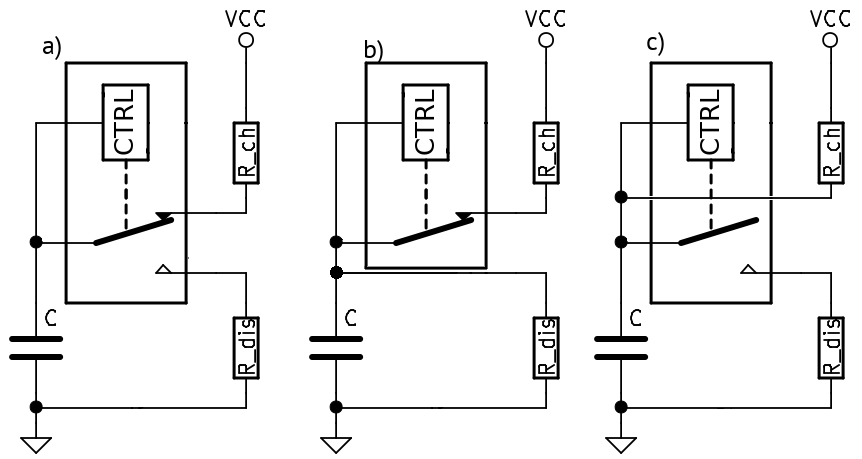
\includegraphics[width=0.8\textwidth]{p/relax_types.png} }
  \caption{Условные схемы релаксационных генераторов.}
  \label{atu:f:relax_types}
\end{figure}

Представленные на рис.~\ref{atu:f:relax_types}
основные виды релаксационных генераторов отличаются
тем, как переключающий элемент (CTRL)
подключает цепи заряда и разряда. А схеме (a)
одновременно подключена только одна из этих цепей.
Такое схемотехническое решение используется достаточно редко.
Схема (b) характеризуется тем, что цепь разряда
подключена постоянно, а цепь разряда
включатся при достижении определённого условия. Такое подключение
характерно для схем импульсных преобразователей и стабилизаторов
напряжения. В схеме (c) наоборот, процесс заряда происходит постоянно,
а разряд -- при условии заданном переключающим элементом. Такое
включение характерно для генераторов пилообразных и других сигналов.
В данной работе в основном будут рассмотрены системы и их модели,
основанные на схеме (с). Принципиальной разницы при использовании
и моделировании других подобных схем не наблюдается.
Существуют и другие схемы, использующие принцип работы
релаксационного генератора, например мультивибраторы,
но исследование их моделей выходит за рамки данной работы.


Основными параметрами схем с релаксационными генераторами являются
напряжения включения $V\Tidx{on}$ и выключения $V\Tidx{off}$
переключающего элемента (CTRL),
напряжение питания $V\Tidx{cc}$,
ёмкость конденсатора $C$,
сопротивления цепей зарядки $R\Tidx{ch}$
и разрядки $R\Tidx{dis}$.
В данной работе, для лучшего проявления
хаотических режимов,
будем полагать, что времена зарядки и разрядки существенно отличаются.
Не снижая общности, считаем, что $R\Tidx{ch} \gg R\Tidx{dis} $.
При предварительном анализе можно считать $R\Tidx{dis} = 0$.
Тем не менее, для обеспечения корректности численного моделирования,
а также обеспечения адекватности модели требуется применение ненулевого значения $R\Tidx{dis}$.
Переменными состояния являются напряжение на конденсаторе $V\Tidx{c}$
и состояние переключающего элемента $\mathrm{On}()$.
В случае использования нескольких релаксационных генераторов
эти величины будем обозначать соответственно как
$V_{i}$ и $ \mathrm{On}_{i}()$.
При этом  $ \mathrm{On}_{i}( V\Tidx{c}, \ldots )$ представляет собой
релейный гистерезисный элемент, обладающий памятью и задаётся алгоритмически.

В этих условиях примем для определённости
(а в большинстве схемотехнических реализаций это так и есть),
что цепь зарядки включена постоянно, а цепь разрядки
включается при $V\Tidx{c} > V\Tidx{on} $ и выключается при
$V\Tidx{c} < V\Tidx{off}$.

С учётом этих обозначений динамика релаксационного генератора
определяется следующим образом:
%
\begin{equation}
  C \od{V_c}{t}
  =
  \frac{V\Tidx{cc} - V\Tidx{c}}{R\Tidx{ch}}
  - \frac{V\Tidx{c}}{R\Tidx{dis}} \cdot \mathrm{On}().
  \label{atu:eq:relax0}
\end{equation}

В случае одного релаксационного генератора
уравнение (\ref{atu:eq:relax0}) можно привести в безразмерному виду,
используя набор очевидных преобразований. В первую
очередь, величина $C R\Tidx{ch}$ определяет
постоянную времени процесса заряда, а процесс
разряда при условии $R\Tidx{ch} \gg R\Tidx{dis} $ будем считать происходящим практически мгновенно.
Обозначим:
%
\begin{equation}
  t_u = \frac{t}{R\Tidx{dis} C} .
  \label{atu:eq:t_u_relax}
\end{equation}

Далее, так как напряжение не опускается ниже $V\Tidx{off}$,
то имеет смысл принять это значение как нулевой потенциал, с соответствующей
коррекцией оставшихся величин. При дальнейшем приведении напряжений к безразмерному виду
можно поступить двумя способами: принять за единицу или
скорректированное напряжение питания $V\Tidx{cc}-V\Tidx{off}$,
или же
скорректированное напряжение включения $V\Tidx{on}-V\Tidx{off}$.
Для одного релаксационного генератора выбор способа практически ни
на что не влияет, но при использовании нескольких --- более удобным
становится первый способ. Таким образом, обозначим:
%
\begin{equation}
  v(t) = \frac{V(t)-V\Tidx{off}}{V\Tidx{cc}-V\Tidx{off}},
  \quad
  v\Tidx{on} = \frac{V\Tidx{on}-V\Tidx{off}}{V\Tidx{cc}-V\Tidx{off}},
  \quad
  v\Tidx{on} \in ( 0; 1 ).
  \label{atu:eq:v_u_relax}
\end{equation}

С учётом этих обозначений, уравнение, описывающее процесс одной зарядки приобретает вид:
%
\begin{equation}
  \od{v}{t_u} = 1 - v( t_u ),
  \quad
  v( t_u ) < v\Tidx{on},
  \quad
  v(0) = 0.
  \label{atu:eq:relax_charge_u}
\end{equation}

Решением (\ref{atu:eq:relax_charge_u}) является
%
\begin{equation}
  v(t_u) = 1 - \exp( - t_u ) ,
  \quad
  v( t_u ) < v\Tidx{on}.
  \label{atu:eq:relax_charge_u_solu}
\end{equation}

Безразмерное время переключения $T_u$,
при пренебрежении временем разрядки,
определяет безразмерный период:
%
\begin{equation}
  v\Tidx{on} = 1 - \exp( - T_u ),
  \quad
  T_u = - \ln ( 1 - v\Tidx{on} ).
  \label{atu:eq:T_u_relax}
\end{equation}

Таким образом, в линейном приближении, и при пренебрежением временем разрядки,
поведение системы определяется одним безразмерным параметром $v\Tidx{on}$,
и определяет другой безразмерный параметр $T_u$.
При $v\Tidx{on} \ll 1 $ процесс зарядки практически линеен,
усреднённое значение $v(t_u)$:
%
\begin{equation}
  \overline{v(t_u)} =
  \frac{1}{T_u}\int\limits_{0}^{T_u} \mathrm{d}t_u
  \approx
  \frac{v\Tidx{on}}{ 2 }.
  \label{atu:eq:av_lin_relax}
\end{equation}
%
и
%
\begin{equation}
  T_u
  \approx
  v\Tidx{on}.
  \label{atu:eq:T_u_lin_relax}
\end{equation}

С другой стороны, при $v\Tidx{on} \to 1$, $T_u \to \infty$,
и
$ \overline{v(t_u)} \to v\Tidx{on}$.
Из этих наблюдений следует, что если для одиночного релаксационного генератора
есть возможность наблюдать период (или же частоту) колебаний,
то безразмерный параметр $v\Tidx{on}$ определяется просто и без
существенных погрешностей измерения. И наоборот,
если для измерения доступна величина $\overline{v(t_u)}$,
то при малых значениях $v\Tidx{on}$ сложностей при измерении (или же идентификации) нет,
а при $v\Tidx{on} \approx 1$ малые изменения $\overline{v(t_u)}$
приводят к практически не ограниченным изменением $T_u$,
что не способствует процессу идентификации.

Тем не менее, в случае, когда в одном генераторе используется
несколько релаксационных элементов,
то понятие периода не имеет особого смысла, или же вообще не
определено в случае хаотического поведения. Поэтому,
измерения усреднённых напряжений может оказаться практически
единственным способом оценки параметров системы.


Если же применяется в одной схеме несколько релаксационных генераторов с различными параметрами,
или же рассматриваются нелинейные зависимости токов от разностей потенциалов,
то приведение к безразмерному виду практического смысла не имеет,
однако закономерности, полученные для простого случая,
полезны для анализа возможных критериев идентификации.


В предыдущих рассуждениях было принято $V\Tidx{cc} = \mathrm{const}$.
Однако, при анализе динамики реальных генераторов
модели, использующие
это предположение,
не вполне адекватно описывают динамику, так как реальные
источники напряжения имеют ограниченные возможности.
При описании одного релаксационного элемента
ограниченность возможностей источника элементарно компенсируется
добавлением внутреннего сопротивления источника к $R\Tidx{dis}$.
В случае, когда один реальный источник питает
насколько генераторов, такой подход становится неприменимым.
В этом случае, для сохранения условия  $V\Tidx{cc} = \mathrm{const}$
будем считать, что эта величина описывает ЭДС источника
без нагрузки, а все релаксационные генераторы
получают от шины питания с напряжением $V_b(t)$,
которое определяется как суммарным током потребления,
так и ограниченным возможностями шины питания,
которые, в первом приближении, описываются
эффективным сопротивлением $R_b$, определяемым как внутренним сопротивлением
источника, так и сопротивлением самой шины, т.е.
%
\begin{equation}
  V_b(t) = V\Tidx{cc} - R_b \sum\limits_{i=0}^{n-1} I_i(t),
  \label{atu:eq:V_b_relax}
\end{equation}
%
где $i$ --- порядковый номер релаксационного элемента,
$I_i(t)$ --- потребляемый им ток.


\section{Свойства и модели переключающего элемента на паре биполярных транзисторов}
\label{atu:sec:relax3d_sw}

Как уже было отмечено, для реализации переключающего элемента релаксационного генератора
существует широкий спектр возможностей. Тем не менее, в рамках данной работы
не ставятся задачи ни анализа работы какого-то определённого элемента,
ни обзора всех существующих. Так как основной задачей данной главы является
синтез системы идентификации для реального генератора, а также
анализ возможности этой системы, то в качестве
переключающих элементов релаксационных генераторов имеет смысл выбирать
те, свойства которых позволяют как с минимальными усилиями,
так и минимальными помехами сопрягать исследуемый генератор
с измерительной системой, реализованной на основе микроконтроллера.
Следовательно, из рассмотрения выпадают газоразрядные лампы,
динисторы, и подобные элементы, требующие относительно
высокого напряжения питания.

Одним из возможных способов реализации переключающего элемента
является схема из двух комплиментарных биполярных транзисторах,
применённая A.S.~Elwakil и M.P.~Kennedy~\cite{kennedy1999}
для создания низковольтного, маломощного хаотического генератора.
Рассмотренная в упомянутой работе схема хаотического генератора
весьма интересна, но включает индуктивный элемент,
что затрудняет создание достаточно точных, и в тоже время простых моделей
из-за сложных трудно воспроизводимых гистерезисных явлений в
ферромагнитном сердечнике. При этом относительно высокий частотный диапазон
затрудняет процесс измерения. Поэтому, в данном исследовании
из этой работы будет использоваться только переключающий элемент~(рис.~\ref{atu:f:relax3d_switch}).

\begin{figure}[htb!]
  \centerline{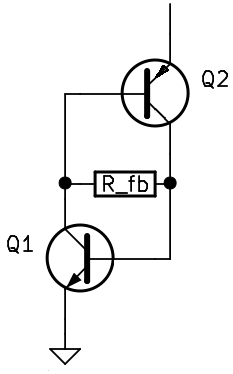
\includegraphics[width=0.25\textwidth]{p/relax3d_switch.png} }
  \caption{Схема переключающего элемента на комплиментарных биполярных транзисторах}
  \label{atu:f:relax3d_switch}
\end{figure}


Результаты численного моделирования работы данной схемы, полученные с помощью
программы моделирования ``ngspice'' 26 представлены на рис.~\ref{atu:f:relax3d_sw_vah}.
Исходная схема была расширена управляемым источником питания и сопротивлением нагрузки $R_n$.
Это позволило получить семейство вольт-амперных характеристик при разных значениях $R_{fb}$.

\begin{figure}[htb!]
  \centerline{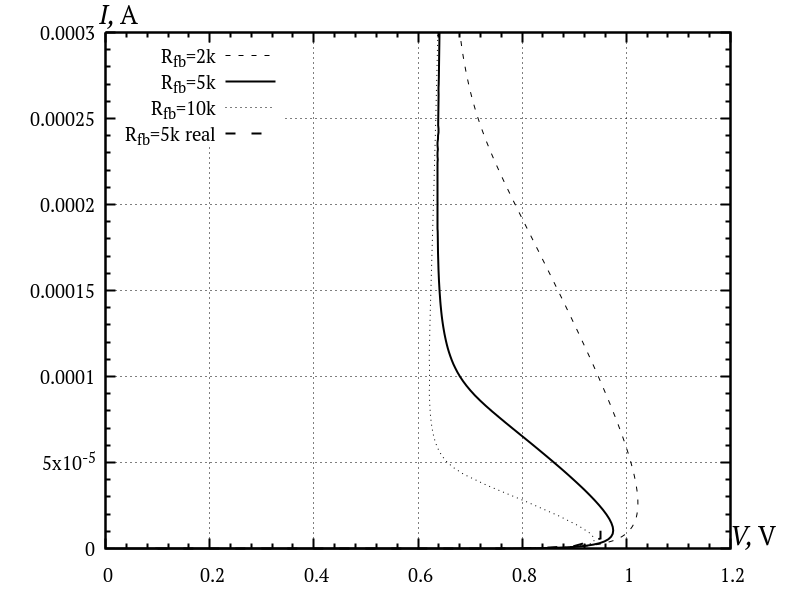
\includegraphics[width=0.6\textwidth]{p/relax3d_sw_va.png} }
  \caption{Семейство расчётных вольт-амперных характеристик переключающего элемента на комплиментарных биполярных транзисторах,
  в сравнении с реальными данными}
  \label{atu:f:relax3d_sw_vah}
\end{figure}

Все вольт-амперные характеристики, полученные путём моделирования,
имеют S-образную форму, характерную для бистабильных
переключающих элементов, таких как динисторы, газоразрядные лампы и т.д.
Участки характеристик, соответствующие отрицательному
дифференциальному сопротивлению, являются неустойчивыми,
и в реальных схемах не реализуются.
Поэтому реальные данные для этих участков не представлены.
То, что эти значения
были получены в программе моделирования,
свидетельствует о недостаточной адекватности применяемых моделей.
Еще одним подтверждением ограниченной адекватности моделей, используемых
в программах для моделирования, основанных на ``spice'',
является тот факт, что в рассмотренных программах из этого семейства
не удалось достичь работоспособности модели релаксационного генератора
с указанным переключающим элементом.

Сложная нелинейная вольт-амперная характеристика рассматриваемого переключающего элемента,
тем не менее, в широком диапазоне параметров,
не служит серьёзным препятствием для моделирования
релаксационного генератора в целом.
Как следует из представленных графиков, ток до момента переключения
не превышает $\SI{2e-6}{\ampere}$, а на значительной части рабочего участка
не превышает $\SI{1e-8}{\ampere}$, что для многих (но не для всех)
условий может рассматриваться как просто выключенное состояние, $I\Tidx{dis}=0$.


С другой стороны, после переключения эффективное сопротивление этого элемента
достаточно мало, $R\Tidx{dis} \approx \SI{20}{\ohm}$,
что для аналитической оценки практически эквивалентно мгновенному разряду,
а для численного моделирования как ошибки в определении $R\Tidx{dis}$
практически на порядок, так и  нелинейная зависимость существенной роли не играют.
Поэтому, при используемых диапазонах параметров, для моделирования данный элемент можно
представить в виде переключающий функции $\mathrm{On}(V)$.
Параметры этой функции -- $V\Tidx{on}$ и $V\Tidx{off}$
можно определить экспериментально. Экспериментально полученная зависимость для $V\Tidx{on}(R_{fb})$
представлена на (рис.~\ref{atu:f:relax3d_bjt_v_onn}), а величина $V\Tidx{off}$
оказалась практически не зависящий от $R_{fb}$.

\begin{figure}[htb!]
  \centerline{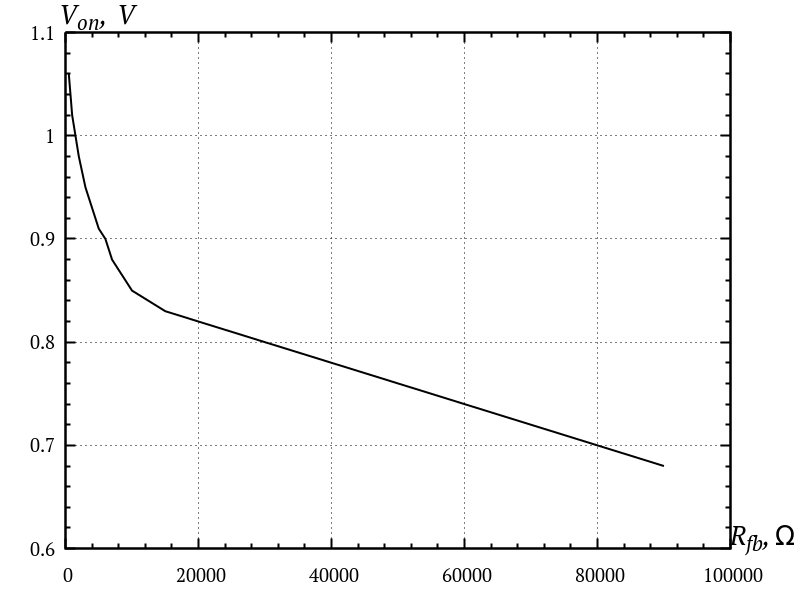
\includegraphics[width=0.7\textwidth]{p/r_fb-V_on.png} }
  \caption{Экспериментальная зависимость $V\Tidx{on}(R_{fb})$ для переключающего элемента на двух комплиментарных биполярных транзисторах}
  \label{atu:f:relax3d_bjt_v_onn}
\end{figure}

Как и для многих электронных схем, использующих свойства p-n переходов,
для данной схемы характерна сильная, практически экспоненциальная зависимость
тока от температуры. В данной работе при проведении экспериментов
разброс температуры не превышал $\SI{5}{\kelvin}$, что позволило
избежать излишнего усложнения модели.

Следует отметить и определённое ограничение при использовании
простой $\mathrm{On}{v}$ модели переключающего элемента.
Для объяснения причины этого ограничения
рассмотрим участки вольт-амперных характеристик,
непосредственно предшествующие переключению (рис.~\ref{atu:f:relax3d_sw_vah_mini}).

\begin{figure}[htb!]
  \centerline{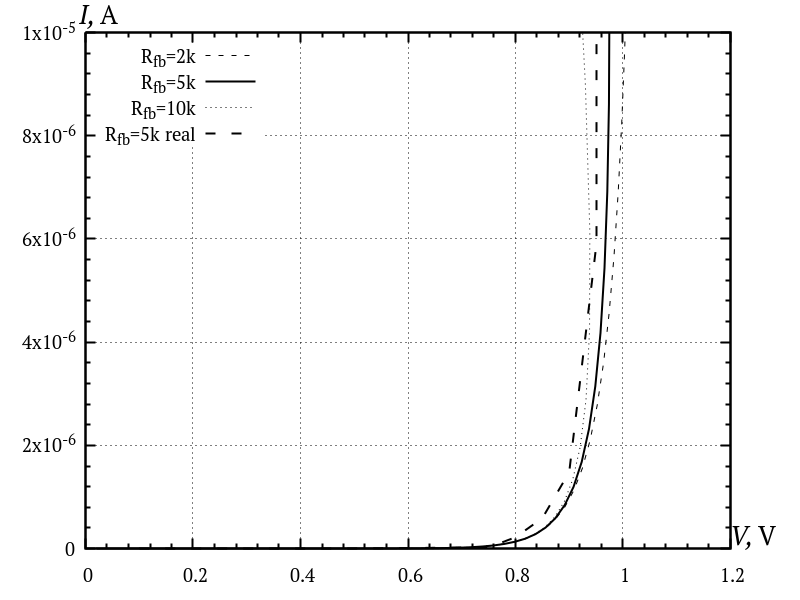
\includegraphics[width=0.6\textwidth]{p/relax3d_sw_va_mini.png} }
  \caption{Участки вольт-амперных характеристик переключающего элемента,непосредственно предшествующие переключению}
  \label{atu:f:relax3d_sw_vah_mini}
\end{figure}

В этих условиях графики похожи на характеристики элементов или же схем,
предназначенных для стабилизации напряжения, т.е. т этих условиях
существенные изменения тока соответствуют малым изменениям падения напряжения.
И если в схеме релаксационного генератора сопротивление $R\Tidx{ch}$ будет настолько
большим, что ток не превысит максимального тока ``стабилизации'',
то напряжение $V\Tidx{on}$ никогда не будет достигнуто,
и генерации колебаний не будет.
Более того, при приближении к этому режиму
адекватность модели будет всё более сомнительна.
Один из способов противостояния ухудшению адекватности
заключается в учёте существенно нелинейной зависимости тока утечки.
Однако, как показали результаты моделирования,
улучшение адекватности хоть и наблюдаются,
но применять такое усложнение модели имеет смысл только в достаточно
узком диапазоне параметров, что не оказывает существенного влияния на
достижение основных целей данной работы.

Таким образом, релаксационный генератор с переключающим
элементом на паре комплиментарных биполярных транзисторов
может использоваться при построении системы связанных генераторов,
а его поведение может быть описано достаточно простой моделью
в широком диапазоне параметров.



\section{Система из трёх связанных релаксационных генераторов на паре комплиментарных транзисторов}
\label{atu:sec:relax3d}


Предлагаемый хаотический генератор представляет собой
систему из трёх релаксационных генераторов,
переключающий элемент в каждом из них реализован
на паре комплиментарных транзисторов~(рис.~\ref{atu:f:relax3d_schem}).

\begin{figure}[htb!]
  \centerline{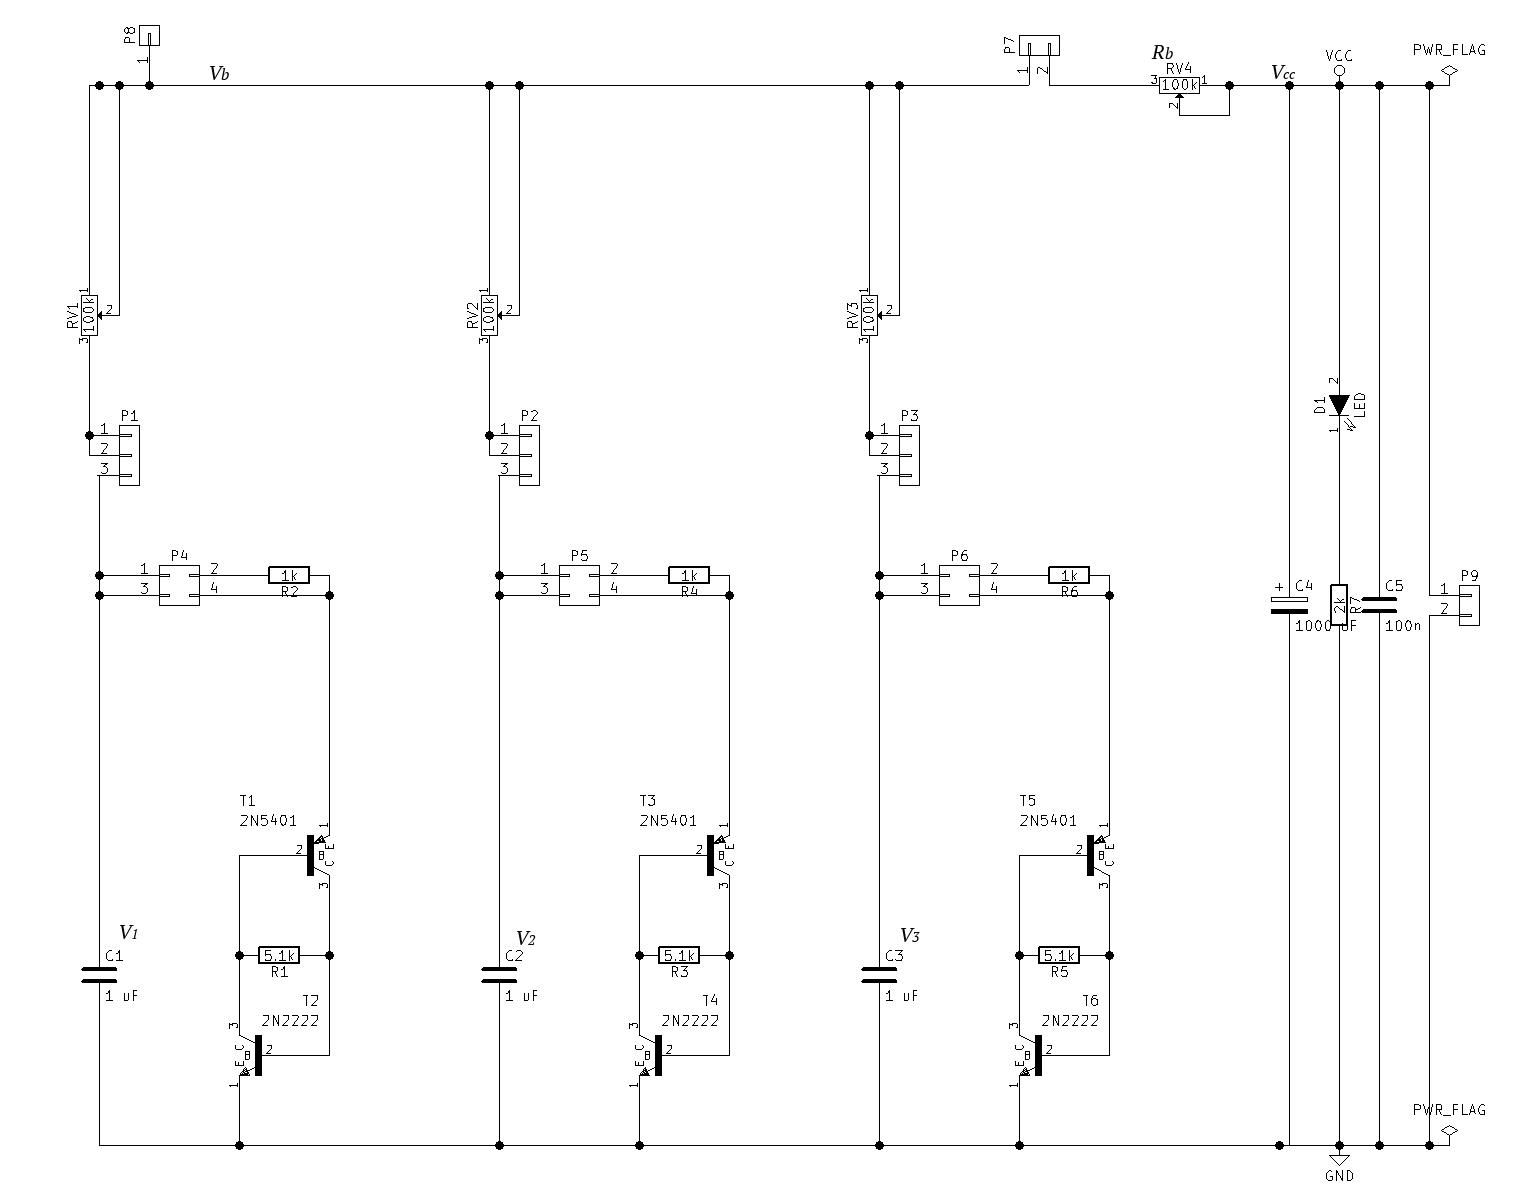
\includegraphics[width=0.96\textwidth]{p/relax3d_schem.png} }
  \caption{Электрическая схема \RelaxBjtIi}
  \label{atu:f:relax3d_schem}
\end{figure}

При создании данной схемы преследовались следующие задачи:
\begin{itemize}

  \item
    работоспособность схемы при малом напряжении питания $V\Tidx{cc}$,
    желательна возможность использования общего питания с микроконтроллером,
    при этом не требуются дополнительные согласующие элементы
    между генератором и АЦП микроконтроллера --- следовательно,
    меньше элементов, которые могут вносить искажения при измерении;

  \item
    относительно низкие рабочие частоты релаксационных генераторов --
    для уменьшения влияния индуктивностей и взаимных связей, не описываемых моделью,
    уменьшению шумов измерения, вызванных искажениями высокочастотных сигналов;

  \item
    возможность оперативно изменять параметры схемы, как отключая отдельные генераторы,
    так и вводя дополнительные элементы.

\end{itemize}

Внешний вид собранной схеме на макетной плате представлен на~(рис.~\ref{atu:f:relax3d_board})

\begin{figure}[htb!]
  \centerline{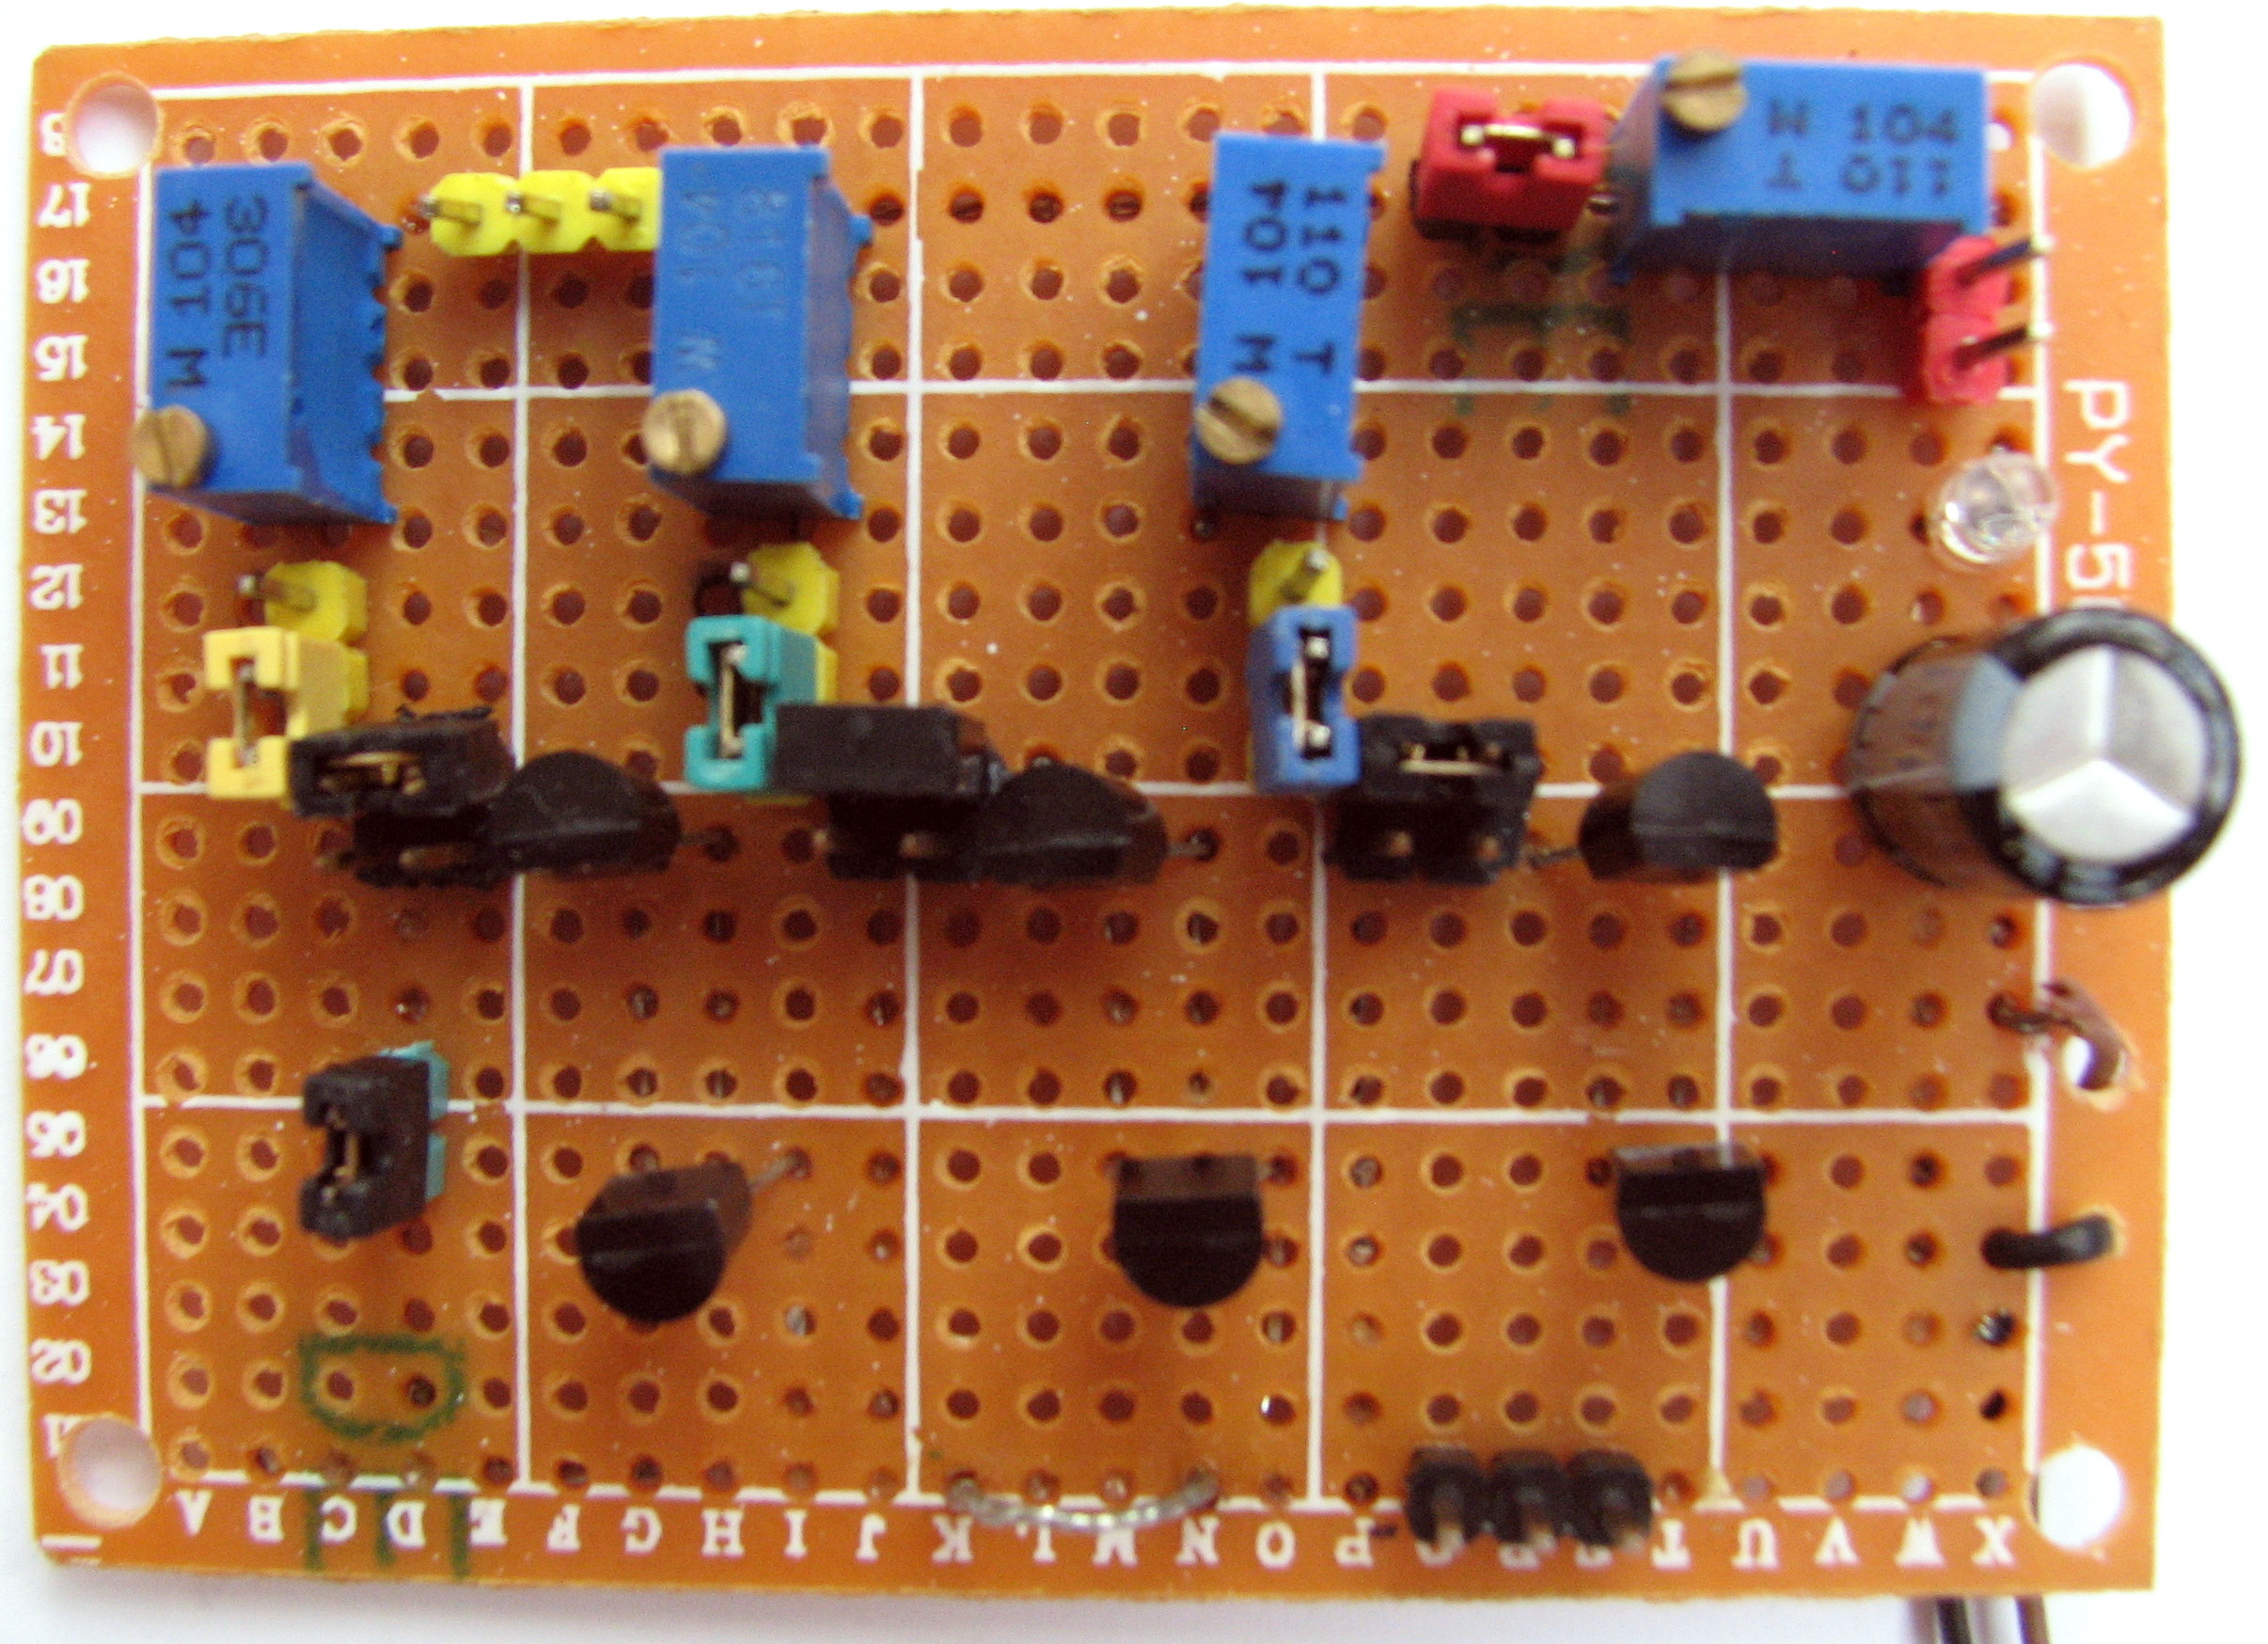
\includegraphics[width=0.6\textwidth]{p/relax3d_board.jpg} }
  \caption{Схема (рис.~\ref{atu:f:relax3d_schem}), собранная на макетной плате}
  \label{atu:f:relax3d_board}
\end{figure}

Данную схемотехническую реализацию в дальнейшем будем обозначать как ``relax3d''.

Возможность работы при низком напряжении питания в данной схеме обеспечивается
применением переключающего элемента с параметрами
$V\Tidx{on} \approx \SI{1.0}{\volt}$,
$V\Tidx{off} \approx \SI{0.6}{\volt}$.
При этом, напряжение питания $V\Tidx{cc} \approx \SI{3}{\volt}$
обеспечивает достаточный диапазон для изменения параметров генератора.
Любое из измеряемых напряжений $V_b$, $V_1$ --- $V_3$
заведомо не превосходит $V\Tidx{cc}$,
что позволяет использовать непосредственную связь
между элементами схемы и АЦП микроконтроллера.
Входные сопротивление каналов АЦП $R\Tidx{measure} \approx \SI{10e7}{\ohm}$
и ёмкость $C\Tidx{measure} \approx \SI{10}{\pico\farad} $
не вносят заметных искажений в работу генератора.

Относительно низкие (десятки и сотни Герц) рабочие частоты
релаксационных элементов были получены путём выбора соответствующих
ёмкостей:
$C_1$ --- $C_3 = \SI{1.0}{\micro\farad}$,
и сопротивлений:
$R_{v1}$ --- $R_{v3} = 1-\SI{100}{\kilo\ohm}$.
Каждое из указанных сопротивлений было подстроечным, для обеспечения
настройки параметров каждого из генераторов. Также подстроечным было сопротивление
$ R_{b} = 1-\SI{100}{\kilo\ohm}$.

Выбранные параметры генераторов определяют небольшой ток
потребления схемы, порядка единиц миллиампер, что
практически не оказывает влияния на работу
системы стабилизации напряжения питания микроконтроллера.
Тем не менее, импульсный характер энергопотребления
релаксационных генераторов может привести
к локальным возмущениям $V\Tidx{cc}$, что
как отрицательно сказывается на точности измерений,
так и снижает адекватность моделей, использующих
константное значение $V\Tidx{cc}$.
Для предотвращения этих явлений шины питания на плате генератора
шунтируется параллельно соединёнными конденсаторами $C_4$ и $C_5$,
соответственно электролитическим и керамическим,
а высокочастотные помехи по шине питания блокируются
ферритовыми бусинками непосредственно на соединительных проводах.

Разъёмы $P_1$ --- $P_3$ на каждом  релаксационном элементе
выполняют по две функции.
Во-первых, они обеспечивают точку для подключения измерительного
оборудования при измерении величин $V_1$--$V_3$.
Во-вторых, они позволяют оперативно
подключать и отключать элементы, как для целей
проверки работоспособности частей генератора,
так и для обеспечения проверки адекватности моделирования
отдельного релаксационного элемента.


Разъёмы $P_4$ --- $P_6$
также выполняют по две функции.
Во-первых, они позволяют управлять сопротивлением
разрядки $R\Tidx{dis}$, вводя дополнительные сопротивления
$R_4$ --- $R_6$.
Во-вторых, с их помощью можно ввести дополнительные,
в том числе нелинейные элементы в цепи разряда.

Разъём $P_7$
предназначен для введения дополнительного,
в том числе автоматически управляемого сопротивления
в цепь шины питания.

Для определения рабочего диапазона значений параметра $R_b$,
а также для получения общей картины динамики рассматриваемой системы
были выбраны (или использованы) следующие значения параметров:
$C_1 = C_2 = C_3 = \SI{1.0}{\micro\farad}$,
$R_{V1} = \SI{21.7}{\kilo\ohm}$,
$R_{V2} = \SI{30.2}{\kilo\ohm}$,
$R_{V3} = \SI{26.5}{\kilo\ohm}$,
$V\Tidx{cc} = \SI{3.03}{\volt}$,
$R_{b} \in [0;50]~ \SI{}{\kilo\ohm}$.
Все постоянные резисторы выбирались из серий с 1\%-ным допуском,
омметры поверялись на резисторах с 0.1\%-ным допуском.
Вольтметры и входные каналы АЦП
поверялись на источнике опорного напряжения (ИОН)
REF5025 (Texas Instruments), обеспечивающим
стабильное напряжение $\SI{2.5}{\volt} \pm 0.1 \%$.
При этом контрольный замер выходного напряжения с ИОН
производился как до, так и после каждой из серий измерений.

При каждом замере
производилась запись величин
$V_b$, $V_1$ --- $V_3$.
Частота дискретизации составляла $\SI{100}{\kilo\hertz}$,
что несколько избыточно для измерения в данном диапазоне.
Как показали последующие измерения,
все значимые в данных экспериментах сигналы не имеют
частот выше $\SI{1}{\kilo\hertz}$,
и представленные спектры будут ограничены этой частотой.
Тем не менее, при моделировании релаксационных
процессов требуется обеспечить требования к устойчивости
самого процесса моделирования, и скачкообразный
характер зависимостей $V_i(t)$
требует уменьшения шага моделирования, и для
рассматриваемой системы частота
$\SI{100}{\kilo\hertz}$ оказалась достаточной.
Для исключения необходимости передискретизации
при сравнении результатов моделирования
и эксперимента была выбрана именно такая частота дискретизации.
Время как измерения, так и моделирования составляло
$\SI{5}{\s}$, что составляет 500000 отчётов
по каждому из каналов.
Эти параметры измерения позволяют получить достаточно
колебаний для построения аттракторов системы.
При этом разрешение в спектральной области
составляет
$\SI{0.2}{\hertz}$, что с учётом погрешностей измерений,
достаточно для разделения сплошного и линейчатого спектров.

Рассмотрим ряд примеров динамики системы
при различных значениях параметра $R_b$.

При малых (относительно $R_{V1}$--$R_{V3}$)
значениях $R_b$
колебания каждого из релаксационных генераторов
происходят практически независимо~(рис.~\ref{atu:f:relax3d_t_02}).

\begin{figure}[htb!]
  \centerline{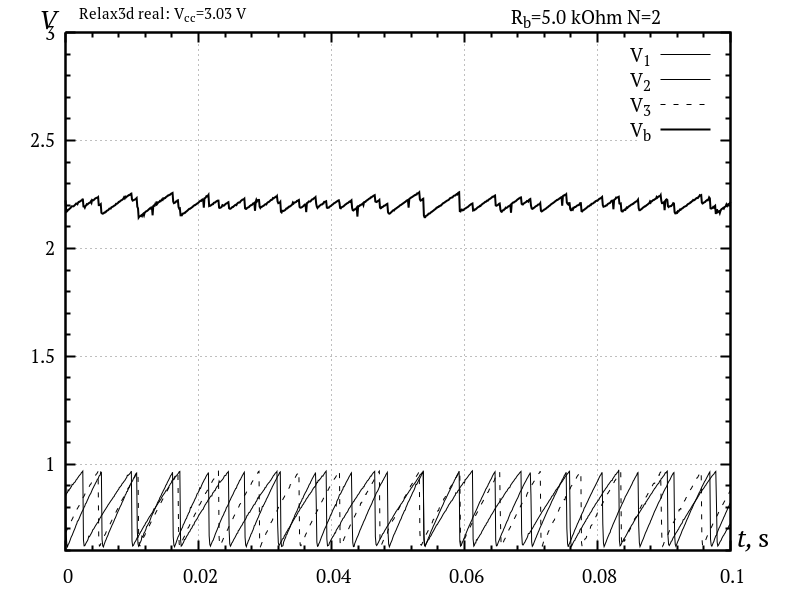
\includegraphics[width=0.6\textwidth]{p/relax3d_t_02.png} }
  \caption{Зависимости $V_b(t)$, $V_i(t)$ для системы ``relax3d'' при $R_b=\SI{5.0}{\kilo\ohm}$ }
  \label{atu:f:relax3d_t_02}
\end{figure}

В этих условиях спектр $V_b(t)$ практически представляет собой линейную комбинацию спектров
(с соответствующими коэффициентами) отдельных релаксационных
элементов, т.е. набор отдельных частот~(рис.~\ref{atu:f:relax3d_f_02},a).
Аттрактор системы при этом имеет вид достаточно нетипичный для
систем, не демонстрирующих хаотическую динамику (рис.~\ref{atu:f:relax3d_f_02},b).
Если отношения частот релаксационных элементов
не представляют собой рациональное число, то аттрактор
представляет собой куб, плотно заполненный по каждой координате в
диапазоне $[ V\Tidx{off} ; V\Tidx{on} ] $.


\begin{figure}[htb!]
  \centerline{
    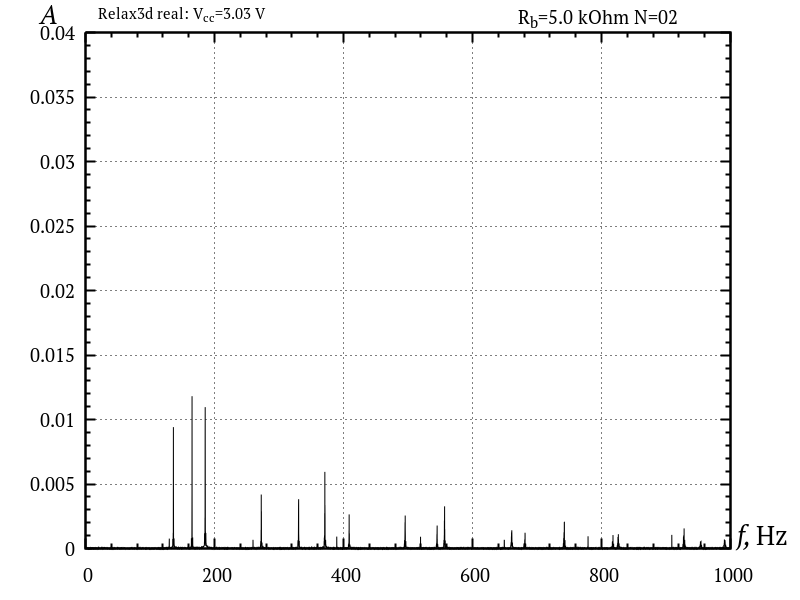
\includegraphics[width=0.48\textwidth]{p/relax3d_f_02.png}
    ~
    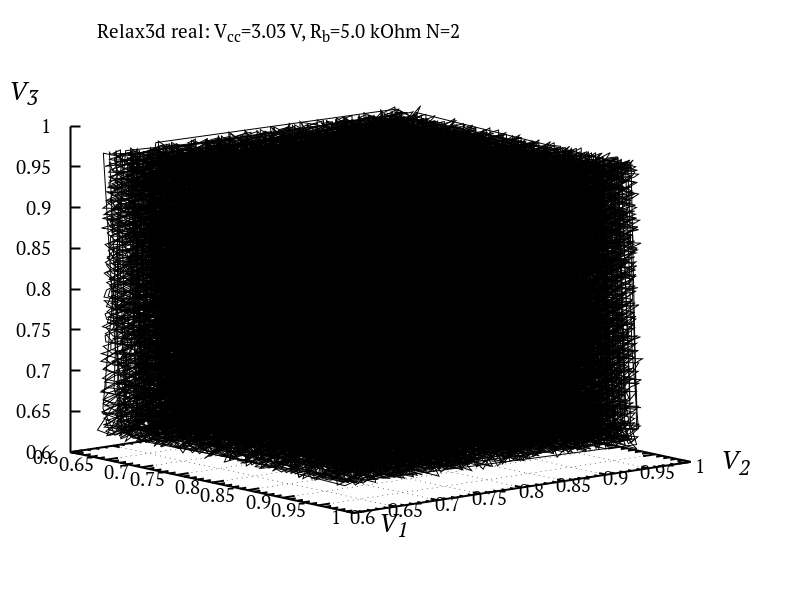
\includegraphics[width=0.48\textwidth]{p/relax3d_v1v2v3_02.png}
  }
  \caption{Спектр $V_b(t)$, и аттрактор для системы ``relax3d'' при $R_b=\SI{5.0}{\kilo\ohm}$ }
  \label{atu:f:relax3d_f_02}
\end{figure}

При увеличении $R_b$ связь между релаксационными элементами становится более сильной
(рис.~\ref{atu:f:relax3d_t_08}), и при этом возможна ситуация, когда
процесс заряда одного элемента настолько замедляет момент переключения другого,
что это замедление влияет на все элементы. Возникает состояние ``гонки'',
когда первый переключившийся элемент существенно замедляет переключение второго.
Таким образом, возникает точка бифуркации, когда малые изменения
в исходном состоянии системы приводят к существенным изменением в последующей динамике.
При благоприятных условиях это может приводить к хаотическому поведению.


\begin{figure}[htb!]
  \centerline{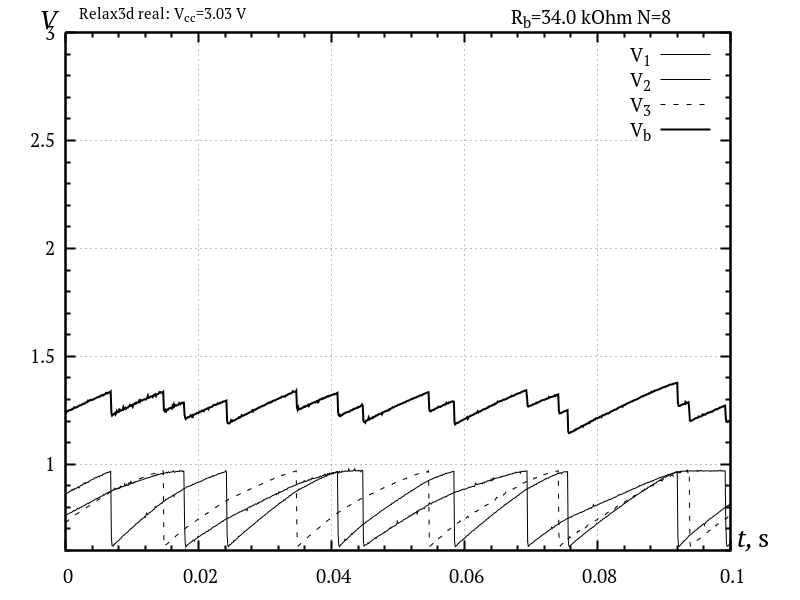
\includegraphics[width=0.6\textwidth]{p/relax3d_t_08.png} }
  \caption{Зависимости $V_b(t)$, $V_i(t)$ для системы ``relax3d'' при $R_b=\SI{34.0}{\kilo\ohm}$ }
  \label{atu:f:relax3d_t_08}
\end{figure}

При этом спектр системы имеет сплошные участки, подтверждая
хаотичность поведения~(рис.~\ref{atu:f:relax3d_f_08},a).
Аттрактор же системы~(рис.~\ref{atu:f:relax3d_f_08},b),
наоборот, менее плотно заполняет доступное пространство.

\begin{figure}[htb!]
  \centerline{
    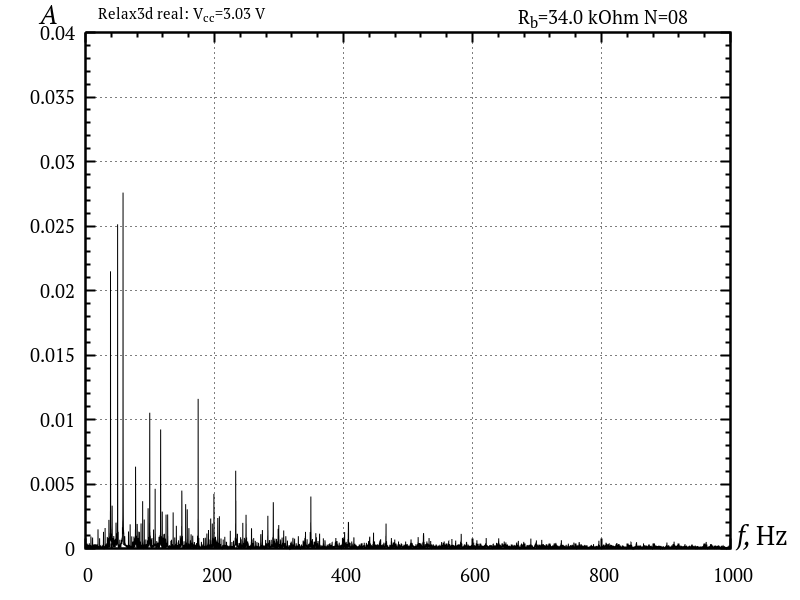
\includegraphics[width=0.48\textwidth]{p/relax3d_f_08.png}
    ~
    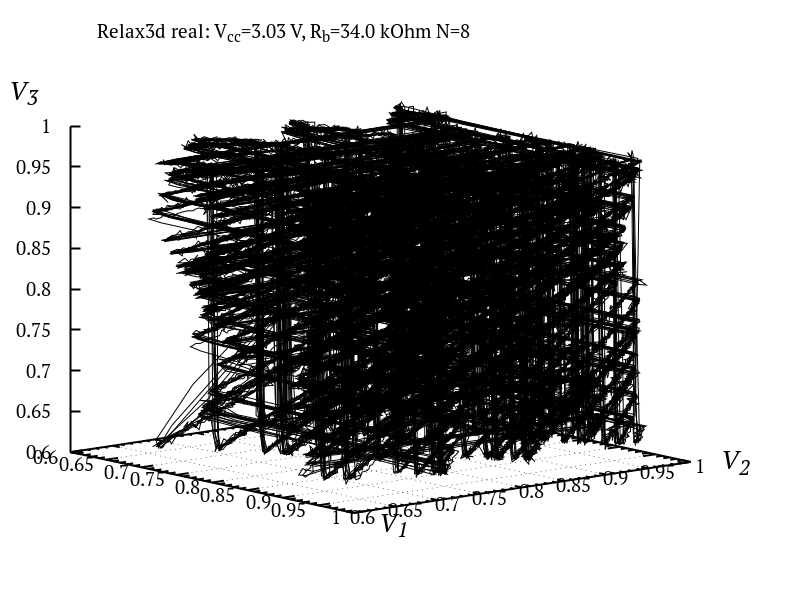
\includegraphics[width=0.48\textwidth]{p/relax3d_v1v2v3_08.png}
  }
  \caption{Спектр $V_b(t)$, и аттрактор для системы ``relax3d'' при $R_b=\SI{34.0}{\kilo\ohm}$ }
  \label{atu:f:relax3d_f_08}
\end{figure}

Однако, сильная связь между релаксационными элементами
совершенно не обязательно приводит к хаотическому поведению.
При определённых условиях возможна самосинхронизация
элементов генератора, то есть создаются условия,
эквивалентные рациональному отношению частот отдельных генераторов.
Например, при дальнейшем увеличении $R_b$, снова
возникает сложно-периодическое поведение~(рис.~\ref{atu:f:relax3d_t_09}).

\begin{figure}[htb!]
  \centerline{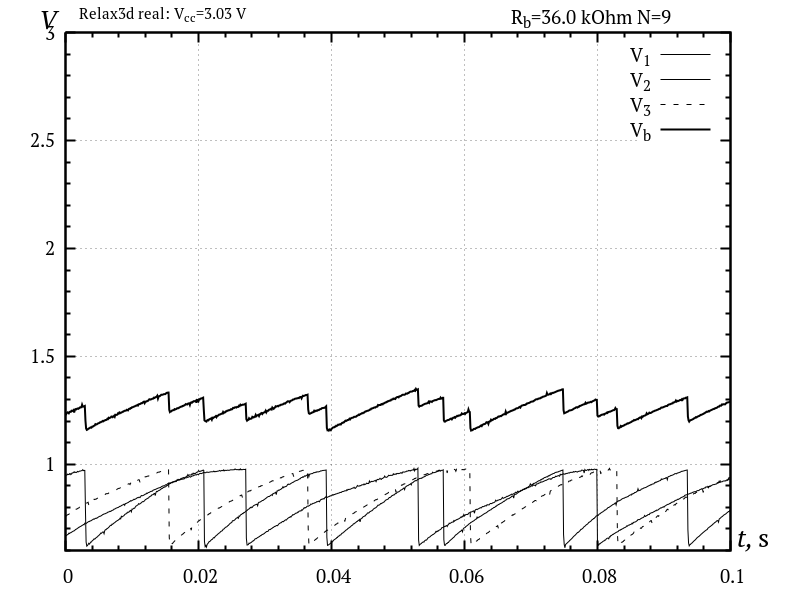
\includegraphics[width=0.6\textwidth]{p/relax3d_t_09.png} }
  \caption{Зависимости $V_b(t)$, $V_i(t)$ для системы ``relax3d'' при $R_b=\SI{36.0}{\kilo\ohm}$ }
  \label{atu:f:relax3d_t_09}
\end{figure}

Спектр системы становится линейчатым (рис.~\ref{atu:f:relax3d_f_09},a), при этом
часто наблюдается равные расстояния между пиками частот.
Аттрактор становится более вырожденным (рис.~\ref{atu:f:relax3d_f_09},b).

\begin{figure}[htb!]
  \centerline{
    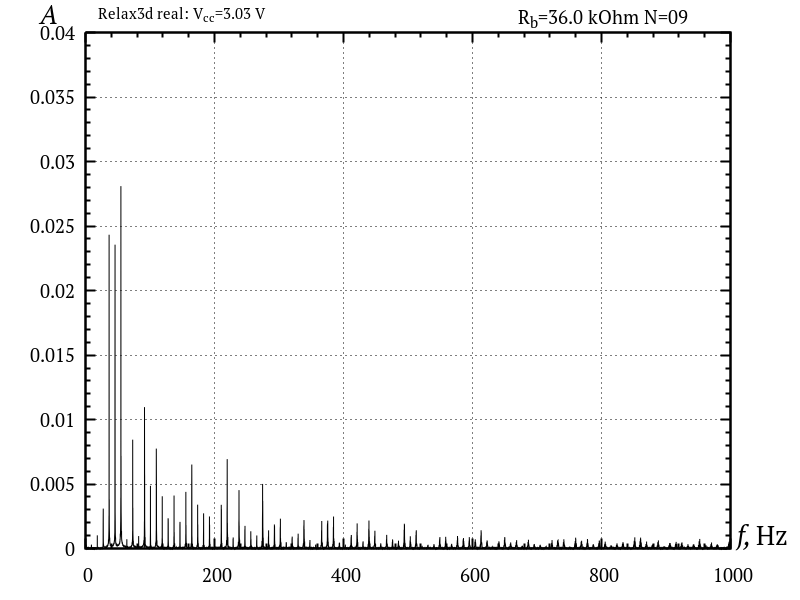
\includegraphics[width=0.48\textwidth]{p/relax3d_f_09.png}
    ~
    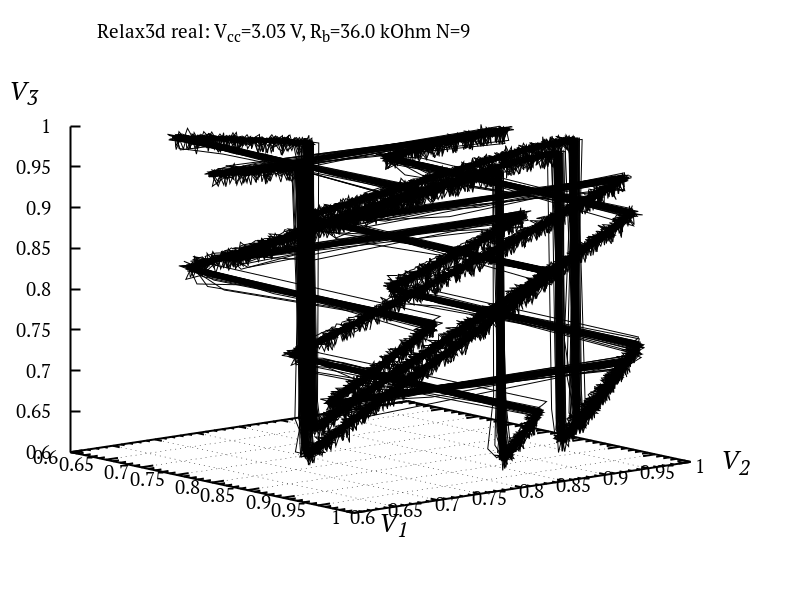
\includegraphics[width=0.48\textwidth]{p/relax3d_v1v2v3_09.png}
  }
  \caption{Спектр $V_b(t)$, и аттрактор для системы ``relax3d'' при $R_b=\SI{36.0}{\kilo\ohm}$ }
  \label{atu:f:relax3d_f_09}
\end{figure}

С дальнейшим ростом значения параметра $R_b$, сложно-периодический и хаотический
режимы чередуются. В конце концов, возникает режим, когда
один из релаксационных элементов прекращает генерацию~(рис.~\ref{atu:f:relax3d_t_22}).
Этот момент наступает значительно раньше, чем предсказывает
модель. Это связано с тем, что применённый в данной схеме переключающий элемент
при малых токах начинает работать как стабилизатор напряжения.

\begin{figure}[htb!]
  \centerline{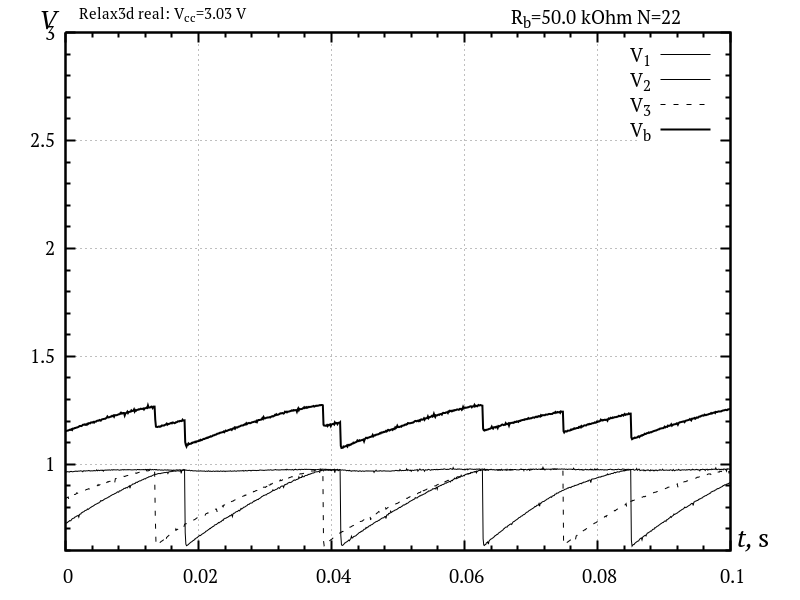
\includegraphics[width=0.6\textwidth]{p/relax3d_t_22.png} }
  \caption{Зависимости $V_b(t)$, $V_i(t)$ для системы ``relax3d'' при $R_b=\SI{50.0}{\kilo\ohm}$ }
  \label{atu:f:relax3d_t_22}
\end{figure}

Оставшиеся два рабочих релаксационных элемента обеспечивают
достаточно бедный линейчатый спектр~(рис.~\ref{atu:f:relax3d_f_22},a).
Аттрактор при этом теряет одно из измерений~(рис.~\ref{atu:f:relax3d_f_22},b),
соответствующее выключившемуся из генерации элементу.

\begin{figure}[htb!]
  \centerline{
    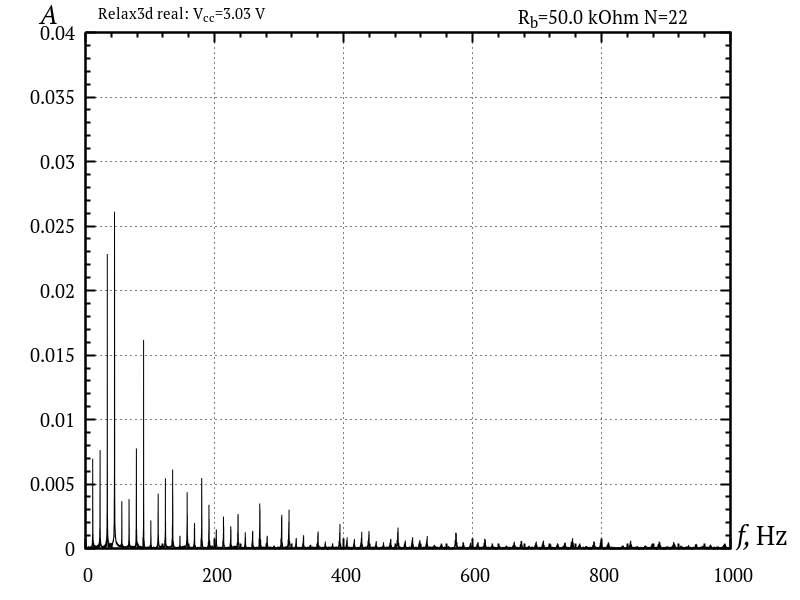
\includegraphics[width=0.48\textwidth]{p/relax3d_f_22.png}
    ~
    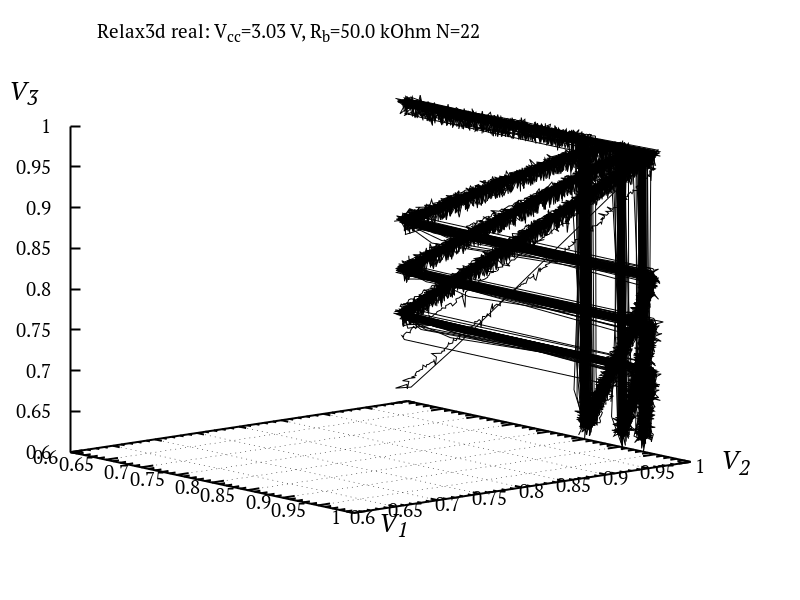
\includegraphics[width=0.48\textwidth]{p/relax3d_v1v2v3_22.png}
  }
  \caption{Спектр $V_b(t)$, и аттрактор для системы ``relax3d'' при $R_b=\SI{50.0}{\kilo\ohm}$ }
  \label{atu:f:relax3d_f_22}
\end{figure}

Таким образом установлено, что
система ``relax3d'', электрическая схема которой приведена на рис.~\ref{atu:f:relax3d_schem},
в интервале значений параметра $R_b \in [1;50]\;\SI{}{\kilo\ohm}$
демонстрирует как сложно-периодическое, так и хаотическое поведение,
причём режимы имеют тенденцию к чередованию.

\section{Система из трёх связанных релаксационных генераторов на основе триггеров Шмидта}
\label{atu:sec:relax3ds}

Схемотехническая реализация системы связанных релаксационных генераторов,
рассмотренная в разделе \ref{atu:sec:relax3d}, несмотря на ряд достоинств,
обладает определёнными недостатками. В первую очередь, следует отметить
тот факт, что при относительно высоких значениях величины $R_b$,
как раз при которых связь между отдельными генераторами становится существенной,
релаксационный элемент переключается из колебательного режима в режим
стабилизации напряжения, что не соответствует предназначению данной схемы.
Более того, в этих условиях зависимость тока от напряжения близка к экспоненциальной,
что затрудняет создание адекватной модели. При этом малые изменения параметров,
например, вызванные температурной нестабильностью, приводят к значительным изменением
тока, что также негативно сказывается на адекватности. Ещё один недостаток
заключается в том, что существующими элементами можно изменять напряжение срабатывания
в достаточно узком диапазоне, что затрудняет проведение как экспериментов,
так и моделирования в широком диапазоне параметров. В свою очередь,
это ставит дополнительные вопросы о границах применимости модели, на которые сложно
ответить, опираясь на результаты эксперимента.

Таким образом, возникает задача синтеза схемы системы связанных
релаксационных генераторов, которая бы в минимальной степени была бы
подвержена вышеупомянутым недостаткам.

Одним из достаточно очевидных способов заключается
в разделении переключающего элемента
на измерительную и переключающую части.
В качестве переключающей части можно продолжить использовать биполярный
транзистор. Использование MOSFET транзистора может позволить
значительно уменьшить сопротивление цепи разряда, однако,
учитывая требование к низкому напряжению питания,
обеспечить полное открытие такого транзистора
без применения специальных драйверов достаточно сложно,
а специальные драйверы требуют отдельного питания,
что требует определённых мер предосторожности при подключении АЦП,
и, в свою очередь, могут вносить дополнительные искажения.

В качестве измерительного элемента можно использовать
подходящую по условиям бистабильную схему,
чувствительную к напряжению, например триггер Шмидта.
Если существует необходимость управлять
значениями величин
$V\Tidx{on}$, $V\Tidx{off}$,
то триггер следует реализовывать,
используя операционные усилители~\cite{horowitz}.
При фиксированных значения этих параметров,
можно использовать триггеры Шмидта в интегральном исполнении,
подобрав соответствующую серию.
У учётом вышеупомянутых требований,
были выбраны микросхемы серии 74HC14N,
представляющие собой 6 элементов ``НЕ''
с триггером Шмидта на входе. Комбинируя их по два,
получим три требуемые измерительные элемента.
Получившаяся схема представлена на рис.~\ref{atu:f:relax3ds_schem}.


\begin{figure}[htb!]
  \centerline{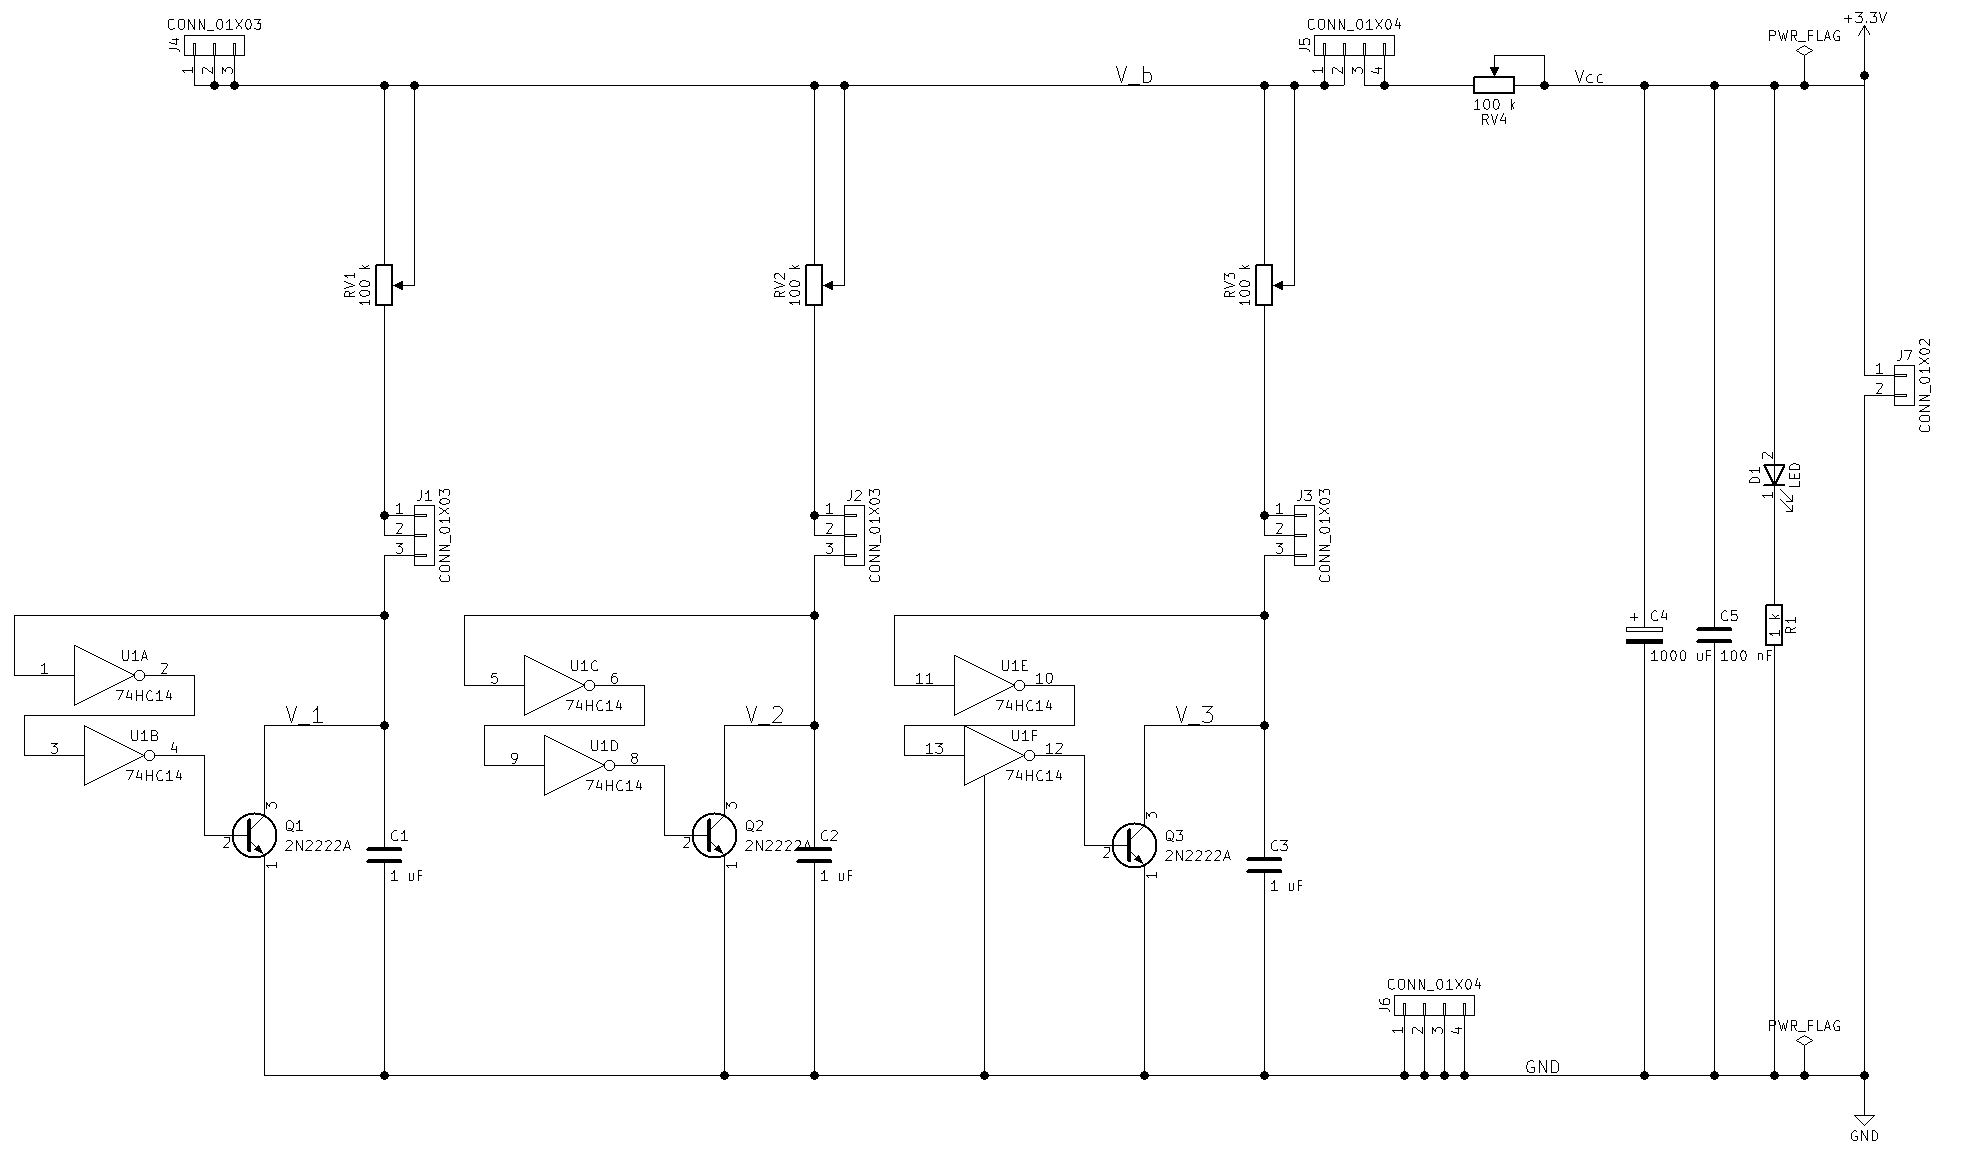
\includegraphics[width=0.9\textwidth]{p/relax3ds_schem.png} }
  \caption{Электрическая схема \RelaxShIi}
  \label{atu:f:relax3ds_schem}
\end{figure}

Принципиальна эта схема не отличается от изображённой на рис.~\ref{atu:f:relax3d_schem}.
Все вспомогательные элементы исполняют аналогичную роль.
При этом существуют и определённые отличия.
Напряжения срабатывания переключающего элемента
у данной схемы отличаются, и определяются
параметрами триггера.
Согласно документации, для указанной микросхемы
при $V\Tidx{cc} = \SI{3}{\volt} $
допустимые диапазоны определяются так:
$V\Tidx{off} \in [ 0.51; 1.35 ]~ \SI{}{\volt}$,
$V\Tidx{on}  \in [ 1.08; 2.16 ]~ \SI{}{\volt}$.
Диапазоны существенно отличаются от таковых для предыдущей схемы.
Более того, разброс допустимых параметров очень широк,
и, теоретически, возможно ситуация, когда некоторые из релаксационных
элементов не будут работать.
Тем не менее, при реальных измерениях
для одного конкретного экземпляра
разброс оказался не так велик:
$V\Tidx{off,1} = \SI{1.10}{\volt}$,
$V\Tidx{off,2} = \SI{1.05}{\volt}$,
$V\Tidx{off,3} = \SI{1.02}{\volt}$,
$V\Tidx{on,1}  = \SI{1.87}{\volt}$,
$V\Tidx{on,2}  = \SI{1.83}{\volt}$,
$V\Tidx{on,3}  = \SI{1.81}{\volt}$.
Различия, несмотря на то, что они заметно меньше, чем допустимы по официальной документации,
тем не менее существенно больше, чем в предыдущей схеме, что требует
обязательного учёта в модели.

Данную схемотехническую реализацию в дальнейшем будем обозначать как ``relax3ds''.

Внешний вид собранной схеме на макетной плате представлен на~(рис.~\ref{atu:f:relax3ds_board})

\begin{figure}[htb!]
  \centerline{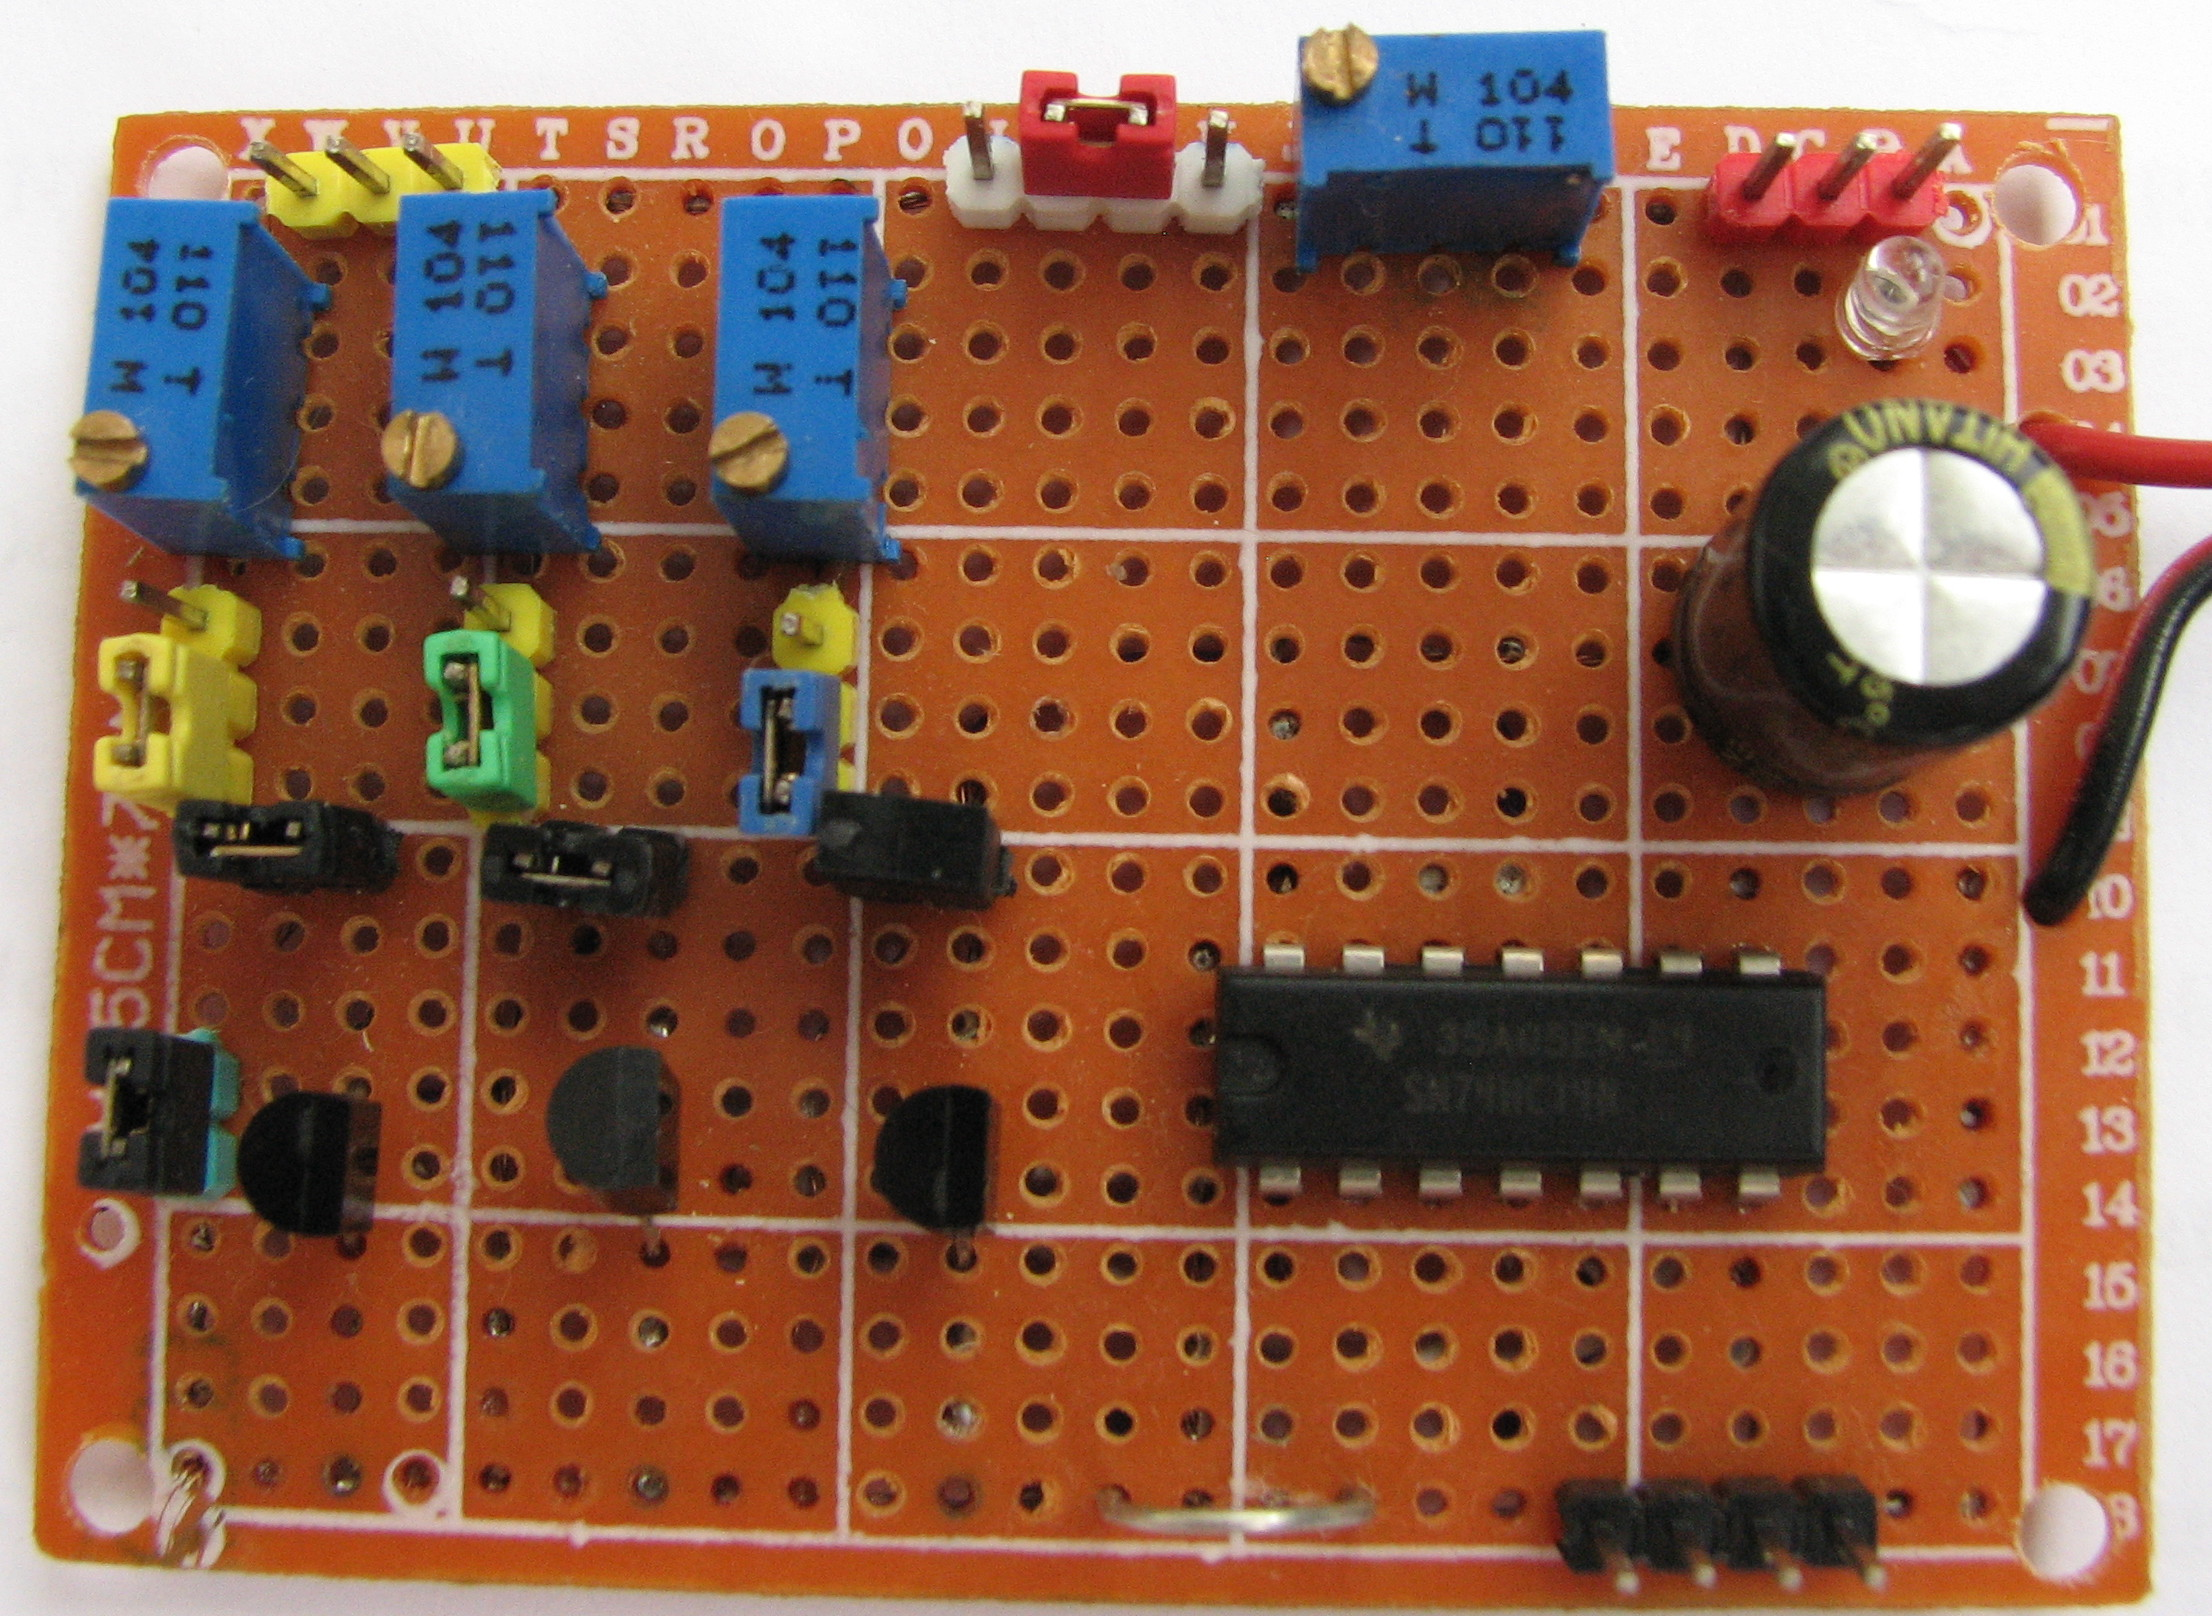
\includegraphics[width=0.6\textwidth]{p/relax3ds_board.jpg} }
  \caption{Схема (рис.~\ref{atu:f:relax3ds_schem}), собранная на макетной плате}
  \label{atu:f:relax3ds_board}
\end{figure}

Аналогично предыдущей схеме, рассмотрим её динамику при
изменении $R_b$, выделяя аналогичные режимы.


При малых
значениях $R_b$
совершенно аналогично наблюдаются практически независимые
колебания~(рис.~\ref{atu:f:relax3ds_t_05151}).
Однако, из-за повышения напряжений переключения,
колебания величины $V\Tidx{b}$
выражены сильнее.

\begin{figure}[htb!]
  \centerline{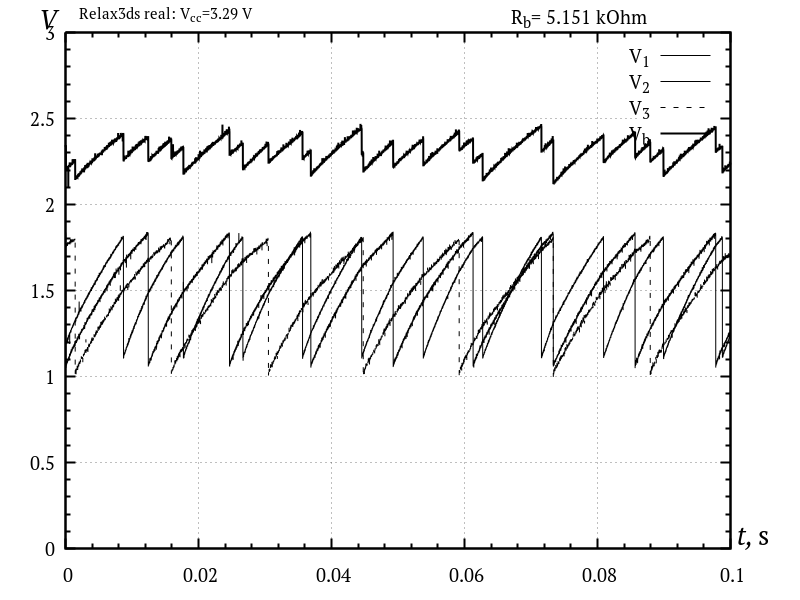
\includegraphics[width=0.6\textwidth]{p/relax3ds_t_005151.png} }
  \caption{Зависимости $V_b(t)$, $V_i(t)$ для системы ``relax3ds'' при $R_b=\SI{5.15}{\kilo\ohm}$ }
  \label{atu:f:relax3ds_t_05151}
\end{figure}


Из-за более сильной связи между элементами,
наблюдается уширение спектральных линий~(рис.~\ref{atu:f:relax3ds_f_05151}).
Аттрактор представляет собой прямоугольный параллелепипед, достаточно плотно заполненный по каждой координате в
диапазоне $[ V\Tidx{off,i} ; V\Tidx{on,i} ] $.


\begin{figure}[htb!]
  \centerline{
    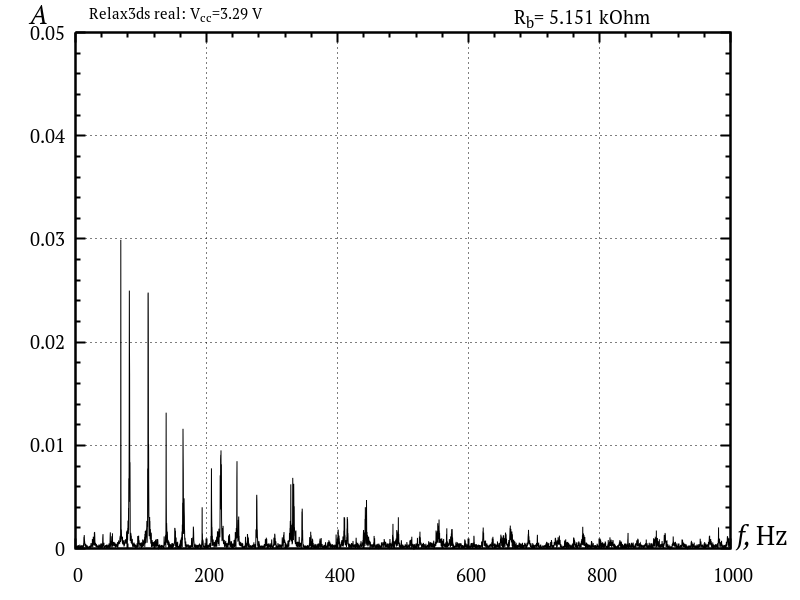
\includegraphics[width=0.48\textwidth]{p/relax3ds_f_005151.png}
    ~
    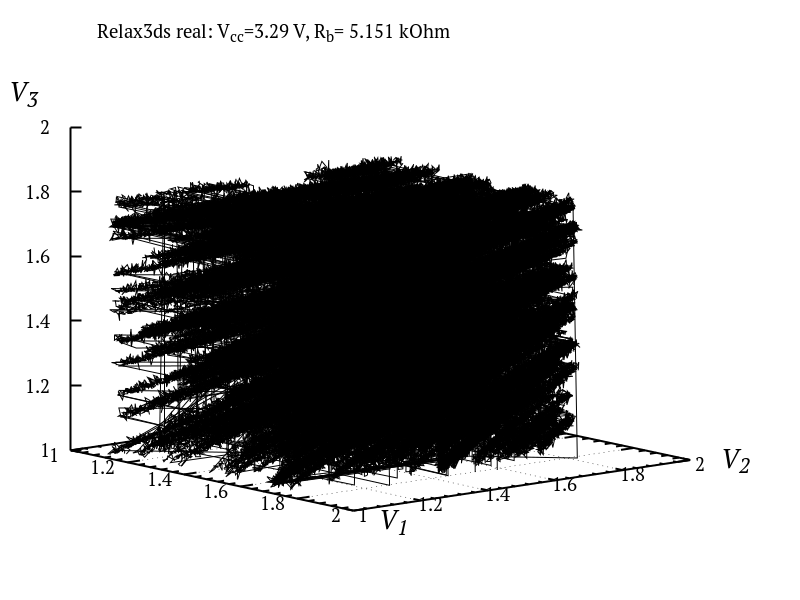
\includegraphics[width=0.48\textwidth]{p/relax3ds_v1v2v3_005151.png}
  }
  \caption{Спектр $V_b(t)$, и аттрактор для системы ``relax3ds'' при $R_b=\SI{5.15}{\kilo\ohm}$ }
  \label{atu:f:relax3ds_f_05151}
\end{figure}

Усиление связи приводит к выраженному хаотическому поведению
(рис.~\ref{atu:f:relax3ds_t_13246}).

\begin{figure}[htb!]
  \centerline{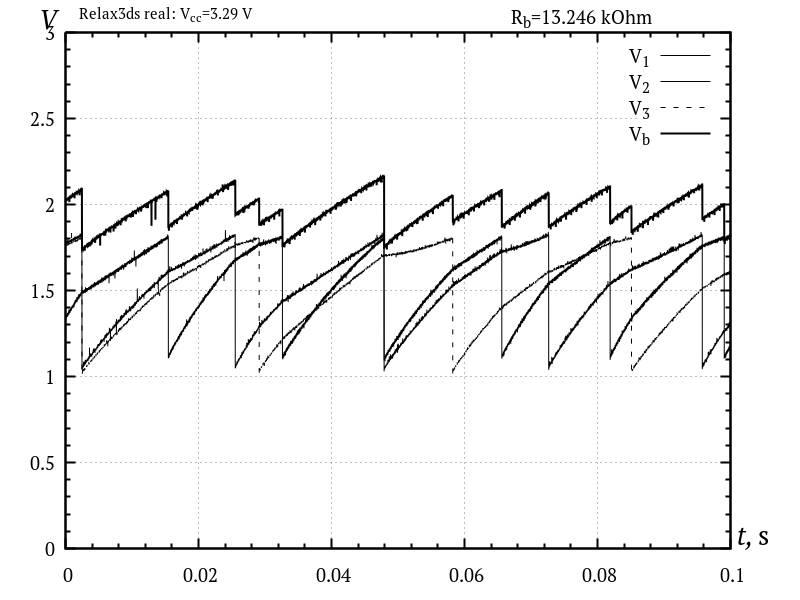
\includegraphics[width=0.6\textwidth]{p/relax3ds_t_013246.png} }
  \caption{Зависимости $V_b(t)$, $V_i(t)$ для системы ``relax3ds'' при $R_b=\SI{13.25}{\kilo\ohm}$ }
  \label{atu:f:relax3ds_t_13246}
\end{figure}

Сплошные участки спектра~(рис.~\ref{atu:f:relax3ds_f_13246},a)
являются хорошим индикатором.
Аттрактор выглядит аналогично~(рис.~\ref{atu:f:relax3ds_f_13246},b).

\begin{figure}[htb!]
  \centerline{
    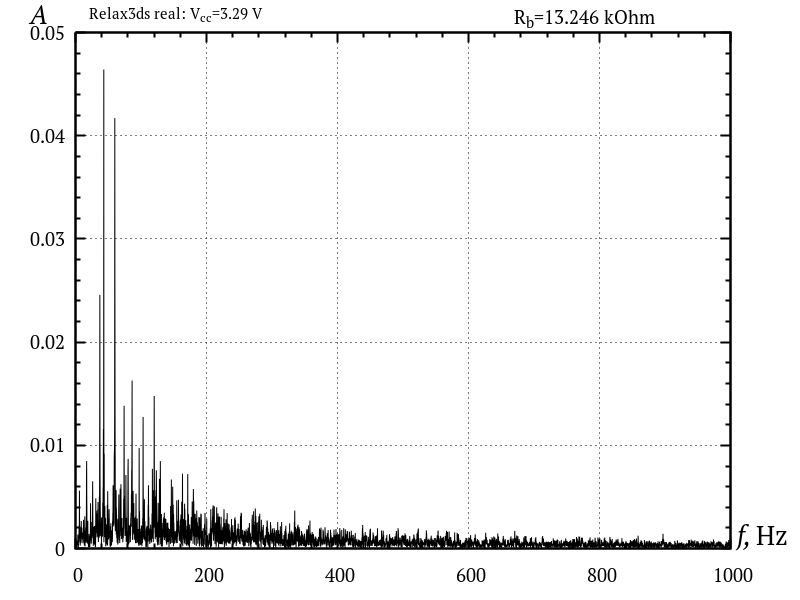
\includegraphics[width=0.48\textwidth]{p/relax3ds_f_013246.png}
    ~
    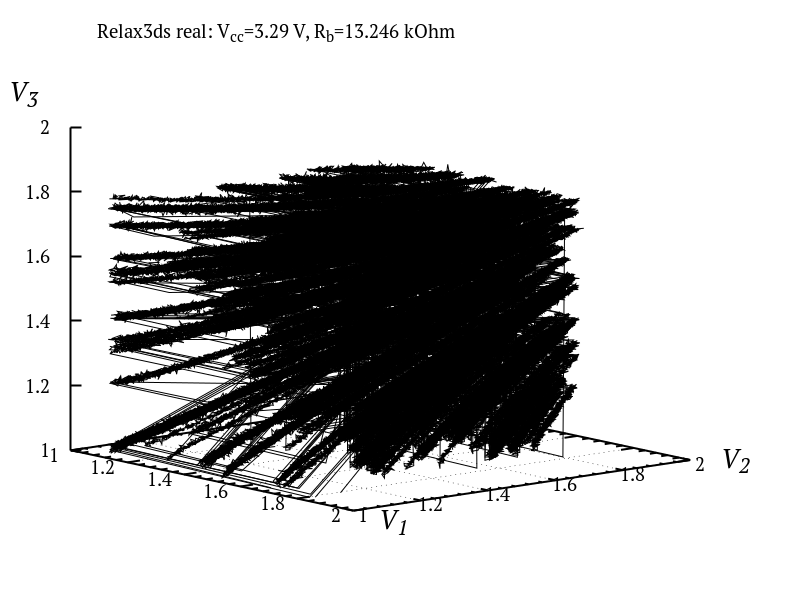
\includegraphics[width=0.48\textwidth]{p/relax3ds_v1v2v3_013246.png}
  }
  \caption{Спектр $V_b(t)$, и аттрактор для системы ``relax3ds'' при $R_b=\SI{13.25}{\kilo\ohm}$ }
  \label{atu:f:relax3ds_f_13246}
\end{figure}


Определённые значения $R_b$ переводят систему в сложно-периодический режим
(рис.~\ref{atu:f:relax3ds_t_14718}).

\begin{figure}[htb!]
  \centerline{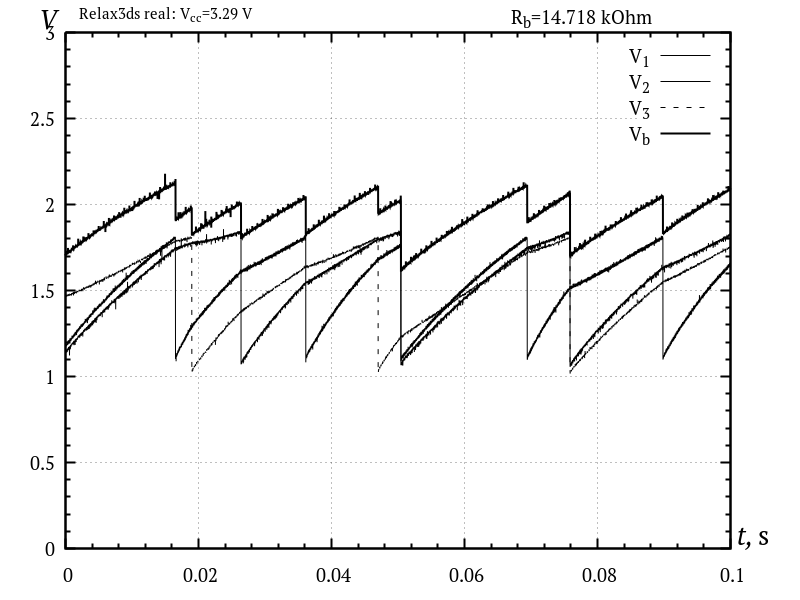
\includegraphics[width=0.6\textwidth]{p/relax3ds_t_014718.png} }
  \caption{Зависимости $V_b(t)$, $V_i(t)$ для системы ``relax3ds'' при $R_b=\SI{14.72}{\kilo\ohm}$ }
  \label{atu:f:relax3ds_t_14718}
\end{figure}

Спектр~(рис.~\ref{atu:f:relax3ds_f_14718},a)
подтверждает отсутствие хаоса,
несмотря на тонкую линейчатую структуру.
Аттрактор принципиально не изменяется~(рис.~\ref{atu:f:relax3ds_f_14718},b),
но имеет менее плотное заполнение.

\begin{figure}[htb!]
  \centerline{
    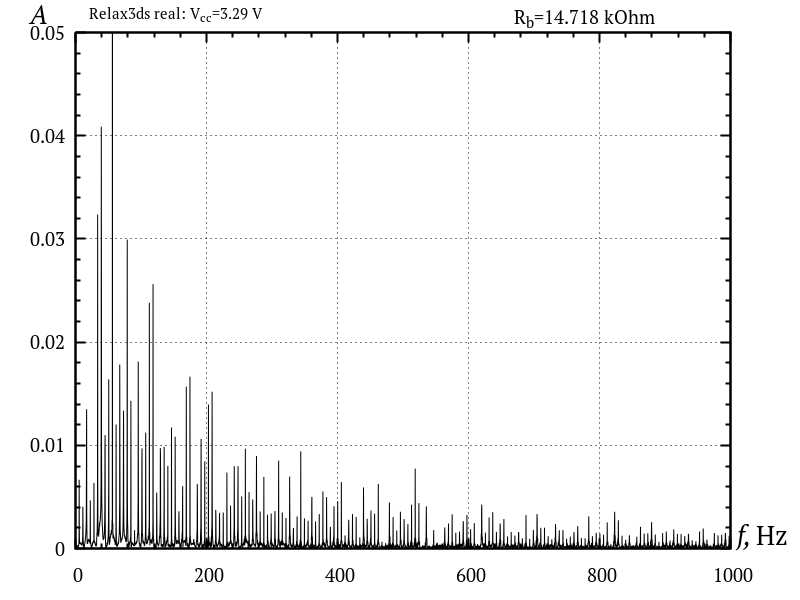
\includegraphics[width=0.48\textwidth]{p/relax3ds_f_014718.png}
    ~
    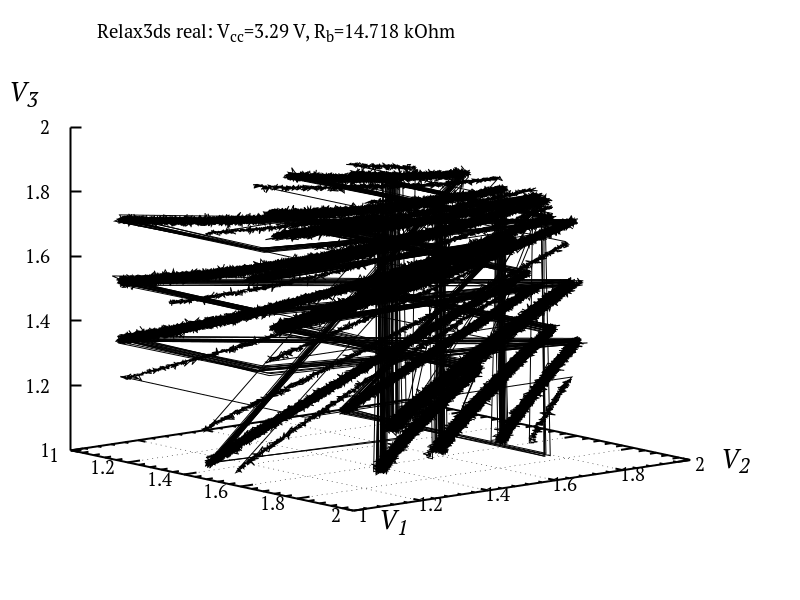
\includegraphics[width=0.48\textwidth]{p/relax3ds_v1v2v3_014718.png}
  }
  \caption{Спектр $V_b(t)$, и аттрактор для системы ``relax3ds'' при $R_b=\SI{14.72}{\kilo\ohm}$ }
  \label{atu:f:relax3ds_f_14718}
\end{figure}

Высокие значения $R_b$, в отличие от предыдущей системы,
не приводят в быстрому выключению одного из релаксационных
элементов, при этом может наблюдаться как сложно-периодическое,
так и хаотическое поведение
(рис.~\ref{atu:f:relax3ds_t_36060}).

\begin{figure}[htb!]
  \centerline{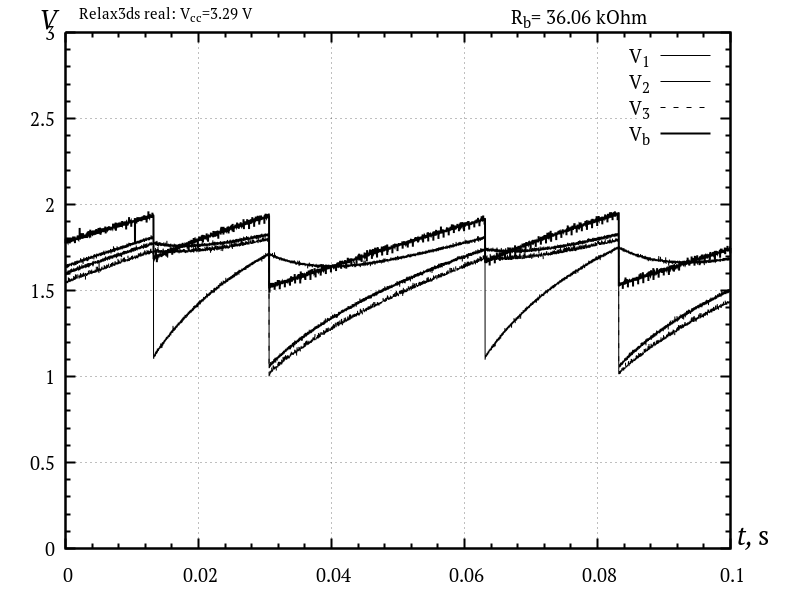
\includegraphics[width=0.6\textwidth]{p/relax3ds_t_036060.png} }
  \caption{Зависимости $V_b(t)$, $V_i(t)$ для системы ``relax3ds'' при $R_b=\SI{36.06}{\kilo\ohm}$ }
  \label{atu:f:relax3ds_t_36060}
\end{figure}

Спектры могут быть как сплошными~(рис.~\ref{atu:f:relax3ds_f_36060},a)
так и линейчатые.
Аттракторы имеют более простую структуру~(рис.~\ref{atu:f:relax3ds_f_36060},b),
при этом реализуя как и простые эквиваленты фигур Лиссажу,
так и фигуры с плотным заполнением.

\begin{figure}[htb!]
  \centerline{
    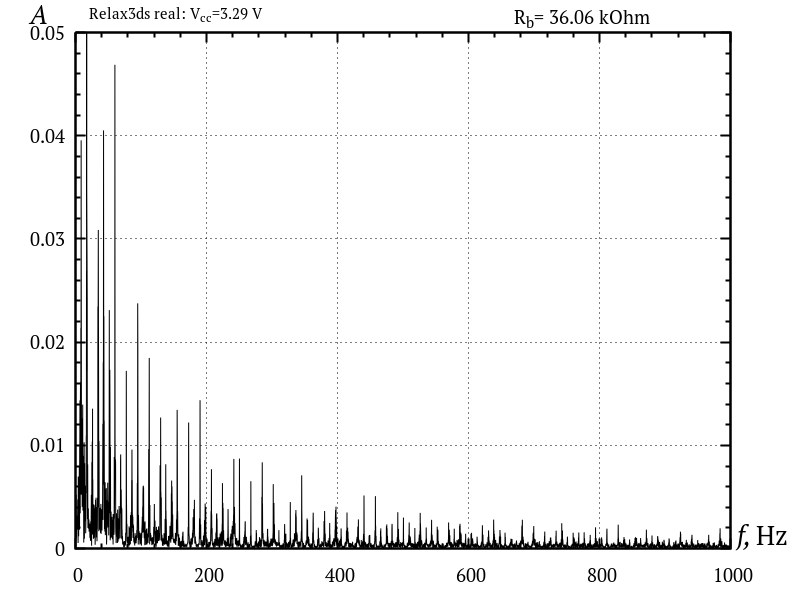
\includegraphics[width=0.48\textwidth]{p/relax3ds_f_036060.png}
    ~
    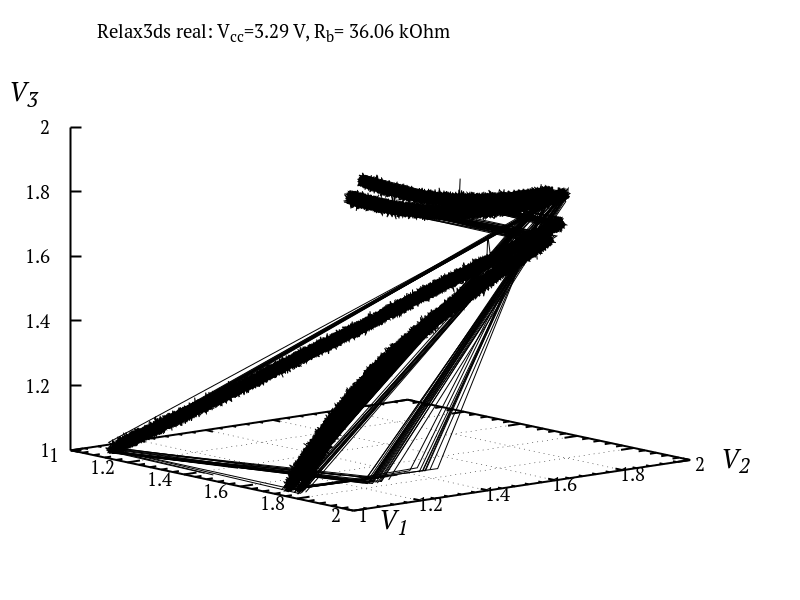
\includegraphics[width=0.48\textwidth]{p/relax3ds_v1v2v3_036060.png}
  }
  \caption{Спектр $V_b(t)$, и аттрактор для системы ``relax3ds'' при $R_b=\SI{36.06}{\kilo\ohm}$ }
  \label{atu:f:relax3ds_f_36060}
\end{figure}

В целом обе схемы, несмотря на различия, имеют сходные принципы поведения
в достаточно широком диапазоне значений параметра $R_b$.
Существенная разница проявляется при высоких значениях $R_b$,
при этом, очевидно, требуется или уточнение модели, или же
не использование данных режимов, которые в этом контексте не представляют
особого интереса.

Сравнение динамики систем ``relax3d'' и ``relax3ds''
позволяет сделать наблюдение,
что при прочих равных первая из них демонстрирует меньший уровень связи между
релаксационными элементами. То есть для получения
аналогичного поведения для второй системы следует задавать меньшие значения $R_b$.
Это связано большим значением безразмерной величины $v$ для второй системы,
из-за относительно больших значений $V\Tidx{off}$, $V\Tidx{on}$.


\section{Модели систем из трёх связанных релаксационных генераторов}

С учётом вышеизложенного, модель системы связанных релаксационных генераторов
можно представить в следующем виде:
%
\begin{equation}
  \begin{cases}
    V_b = V_{cc} - R_b ( I_1 + I_2 + I_3 ), \\
      C_1 \dot{V}_1 = \frac{V_b-V_1}{R_{v1}} - \frac{V_1}{R_1} \mathrm{On}_1() - I_{1,\mathrm{leak}}(V_1), \\
      C_2 \dot{V}_2 = \frac{V_b-V_2}{R_{v2}} - \frac{V_2}{R_2} \mathrm{On}_2() - I_{2,\mathrm{leak}}(V_2), \\
      C_3 \dot{V}_3 = \frac{V_b-V_3}{R_{v3}} - \frac{V_3}{R_3} \mathrm{On}_3() - I_{3,\mathrm{leak}}(V_3), \\
      I_i = \frac{V_b-V_i}{R_{vi}}.
  \end{cases}.
    \label{atu:eq:relax3}
\end{equation}
%
где: \\
$R_b$ --- сопротивление в цепи питания (идентифицируемый параметр), \\
$C_i$ --- ёмкости каждого из релаксационных генераторов, \\
$R_{vi}$ --- сопротивления зарядки релаксационных генераторов, \\
$R_{i}$ --- сопротивления зарядки релаксационных генераторов, \\
$I_{i,\mathrm{leak}}$ --- токи утечки.

Функции $ \mathrm{On}_i() $ определяют моменты срабатывания переключающих элементов,
и ввиду их релейно-гистерезисного вида
задаются алгоритмически. Определяющими параметрам при этом являются
$V_{\mathrm{on},i}$, $V_{\mathrm{off},i}$.

В общем случае токи утечки $I_{i,\mathrm{leak}}$ описываются нелинейными функциями.
В простейших случаях утечку можно моделировать как омическое сопротивление:
%
\begin{equation}
  \begin{cases}
    V_b = V_{cc} - R_b ( I_1 + I_2 + I_3 ), \\
      C_1 \dot{V}_1 = \frac{V_b-V_1}{R_{v1}} - \frac{V_1}{R_1} \mathrm{On}_1() - \frac{V_1}{R_1+R_{1,\mathrm{leak}}}, \\
      C_2 \dot{V}_2 = \frac{V_b-V_2}{R_{v2}} - \frac{V_2}{R_2} \mathrm{On}_2() - \frac{V_2}{R_2+R_{2,\mathrm{leak}}}, \\
      C_3 \dot{V}_3 = \frac{V_b-V_3}{R_{v3}} - \frac{V_3}{R_3} \mathrm{On}_3() - \frac{V_3}{R_3+R_{3,\mathrm{leak}}}, \\
      I_i = \frac{V_b-V_i}{R_{vi}}.
  \end{cases}.
    \label{atu:eq:relax3_linleak}
\end{equation}
%
где
$R_{i,\mathrm{leak}}$ --- сопротивления утечки.
При этом довольно часто выполняется соотношение
$R_{i} \ll R_{i,\mathrm{leak}} $, и величинами
$R_{i}$ можно пренебречь. При выполнении условий
$V_b \gg V_i$ токами утечки можно пренебречь совсем,
однако для хаотических режимов выполнение этого условия нехарактерно,
так как оно подразумевает слабую связь между генераторами.
Конкретный вид утечки следует выбирать, исходя из поведения системы
при условии $V_b \approx V_i$.

Перед тем, как приступить к моделированию системы из связанных генераторов,
необходимо было убедится, что результаты численного моделирования
показывают адекватные результаты в том случае,
когда возможно сравнить результаты не только с экспериментом,
но и с теоретическими расчётами, то есть для одного генератора.
Для проведения этой проверки в системе ``relax3d''
были отключены второй и третий генераторы. При этом, нет необходимости
отслеживать сигнал $V_b(t)$, и в этом эксперименте под величиной
$R_1$ будет подразумеваться сумма $R_1 + R_b$.

При проведении проверки адекватности была проведена серия экспериментов для
одного генератора ``relax1d''
при различных значения $R_1$. В первую очередь было проведено визуальное сравнение
сигналов $V_{1o}(t)$ и $V_{1m}(t)$. Результаты сравнения (пример см.~рис.~\ref{atu:f:relax1d_read_cmp-p_t_r1})
с одной стороны, показывают, что в целом, форма сигналов сигналов достаточно хорошо совпадают,
с учётом разности фаз, которая в реальном эксперименте никак не контролировалась. С другой стороны,
этот график позволяет определить уровень шумов измерения, размах которых
составляет порядка $\SI{20}{\milli\volt}$, что для рассматриваемых условий
является вполне допустимым. Безразмерная величина $v\Tidx{on}$,
характеризующая нелинейность процесса (\ref{atu:eq:v_u_relax}),
составила $0.128$, что подтверждается близким к линейному графику процесса зарядки.



\begin{figure}[htb!]
  \centerline{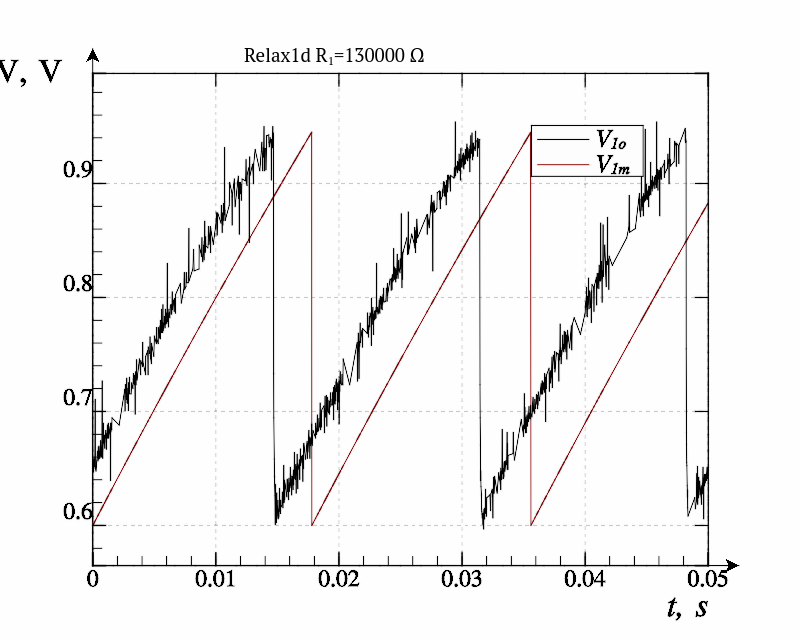
\includegraphics[width=0.6\textwidth]{p/relax1d_read_cmp-p_t_r1=130k.png} }
  \caption{Зависимости $V_1(t)$ полученные в реальном эксперименте ``relax1d'', в сравнении результатами моделирования при $R_1=\SI{130}{\kilo\ohm}$ }
  \label{atu:f:relax1d_read_cmp-p_t_r1}
\end{figure}

Полученная форма сигнала также свидетельствует о том, что можно использовать
как понятие частоты, так и периода сигнала. Вид спектров полученных в результате
эксперимента имеет явно набор ярко выраженных частот (рис.~\ref{atu:f:relax1d_f_r1}),
при этом первый пик и определяет частоту, и соответственно, период сигнала.
При этом, для получения этих значений совершенно не обязательно
проводить достаточно затратный Фурье-анализ сигнала --- достаточно
измерить время, в которое укладывается достаточно большое количество периодов.

\begin{figure}[htb!]
  \centerline{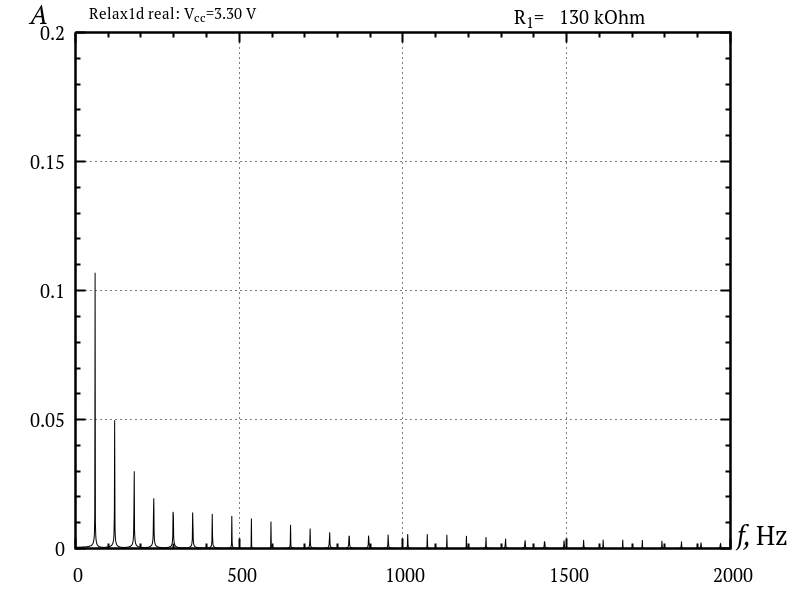
\includegraphics[width=0.6\textwidth]{p/relax1d_f_r1=130k.png} }
  \caption{Спектр сигнала $V_1(t)$ полученного в реальном эксперименте ``relax1d'' при $R_1=\SI{130}{\kilo\ohm}$}
  \label{atu:f:relax1d_f_r1}
\end{figure}

При этом появляется возможность сравнения периодов не только
экспериментальных и модельных результатов, но и полученных
теоретически (\ref{atu:eq:T_u_relax}) при достаточно жёстких ограничениях.


\begin{figure}[htb!]
  \centerline{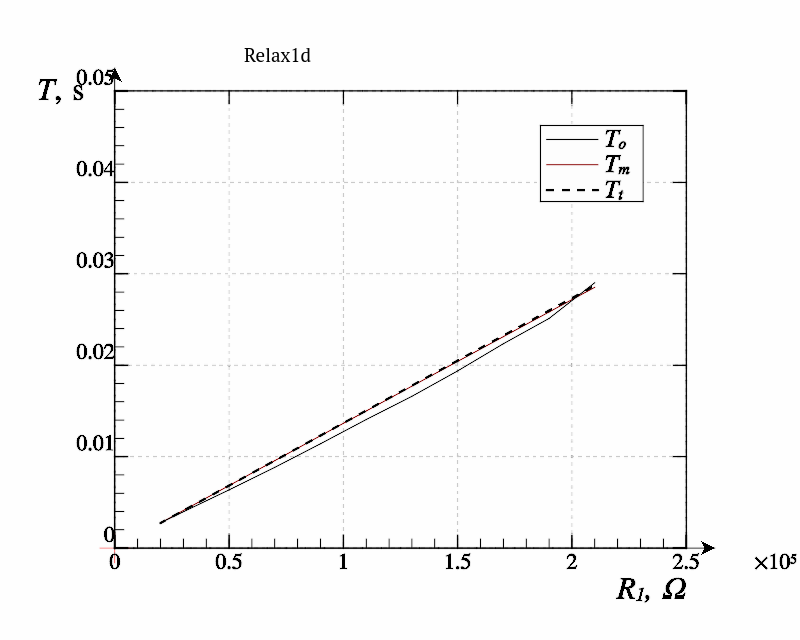
\includegraphics[width=0.6\textwidth]{p/relax1d_read_cmp-p_R1_T.png} }
  \caption{Зависимости $T(R_1)$ в реальном эксперименте ``relax1d'', полученной в результате моделирования, и теоретической (\ref{atu:eq:T_u_relax})}
  \label{atu:f:relax1d_read_cmp-p_R1_T}
\end{figure}

% TODO: more R_1: measure again

Как видно из графиков, (рис.~\ref{atu:f:relax1d_read_cmp-p_R1_T}) результаты
численного моделирования практически полностью совпадают с теоретически
предсказанными. Отличие от эксперимента при этом не превышает 5\%,
что достаточно неплохо, учитывая множество неучтённых в модели факторов.
Таким образом, для одного генератора
модель даёт хорошее совпадение с экспериментом, и может использоваться для
дальнейших исследований.

При росте $R_1$ до величины порядка $\SI{420}{\kilo\ohm}$
наблюдался срыв генерации и переход в режим стабилизации.
Экстраполируя полученные результаты, можно ожидать,
что в системе с тремя такими генераторами аналогичные явления должны наблюдаться
при $R_b \approx \SI{100}{\kilo\ohm}$.

При использовании в качестве переключающего элемента одного генератора
триггера Шмидта (обозначим как ``relax1ds''), были получены аналогичные результаты,
но с определёнными отличиями. Форма колебаний
имеет менее линейный вид, что обусловлено несколько большим значением
безразмерной величины $v\Tidx{on} \approx 0.3$.

\begin{figure}[htb!]
  \centerline{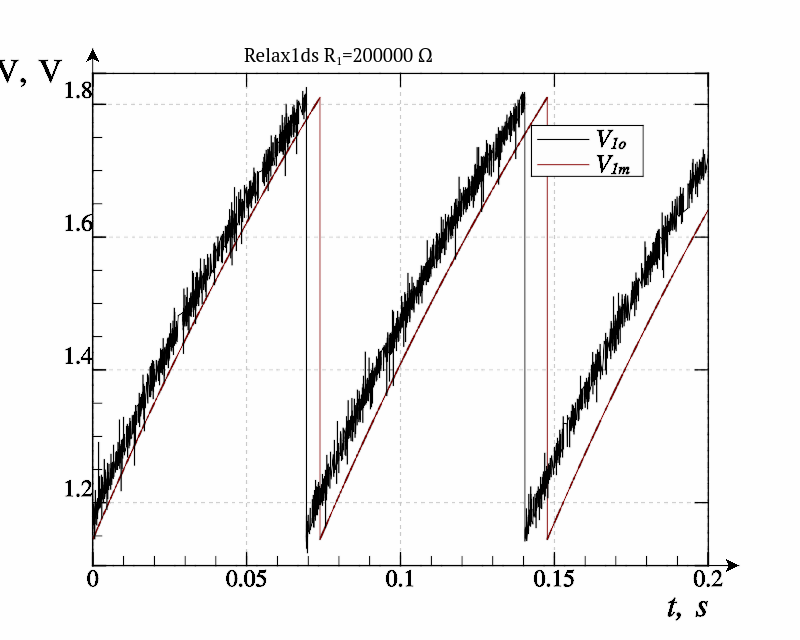
\includegraphics[width=0.6\textwidth]{p/relax1ds_read_cmp-p_t_r1=200k.png} }
  \caption{Зависимости $V_1(t)$ полученные в реальном эксперименте ``relax1ds'', в сравнении результатами моделирования при $R_1=\SI{200}{\kilo\ohm}$ }
  \label{atu:f:relax1ds_read_cmp-p_t_r1}
\end{figure}

Спектр сигнала $V_1(t)$ имеет совершенно аналогичный вид (рис.~\ref{atu:f:relax1ds_f_r1}),
за исключением того, что из-за большего доступного значения $R_1$,
а следовательно, меньшей частоты, относительная разрешающая способность
численного преобразования Фурье оказалась меньше, чем в предыдущем случае.
Тем не менее вид спектра позволяет определить и измерить период.

\begin{figure}[htb!]
  \centerline{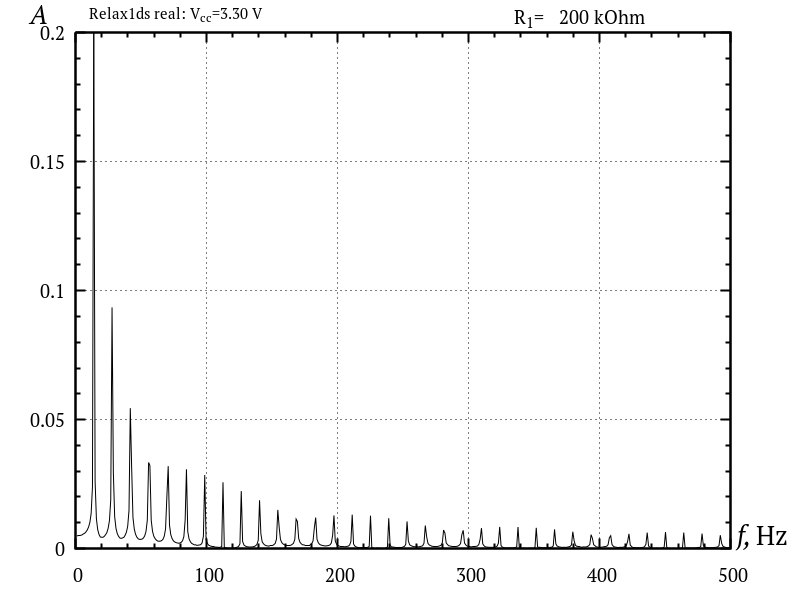
\includegraphics[width=0.6\textwidth]{p/relax1ds_f_200000.png} }
  \caption{Спектр сигнала $V_1(t)$ полученного в реальном эксперименте ``relax1ds'' при $R_1=\SI{200}{\kilo\ohm}$}
  \label{atu:f:relax1ds_f_r1}
\end{figure}

Существенным отличием данного генератора от схемы с двумя биполярными транзисторами
является тот факт, что не происходит срыв генерации при существенном росте $R_1$.
В экспериментах генерация наблюдалась даже при $R_1 = \SI{9}{\mega\ohm}$,
что практически не отличается от входного сопротивления измерительных цепей.
Поэтому, следующий график представлен для существенно большего диапазона величины $R_1$.

Зависимости экспериментального, модельного и теоретического периодов
от величины $R_1$ представлены на рис.~\ref{atu:f:relax1ds_read_cmp-p_R1_T}.


\begin{figure}[htb!]
  \centerline{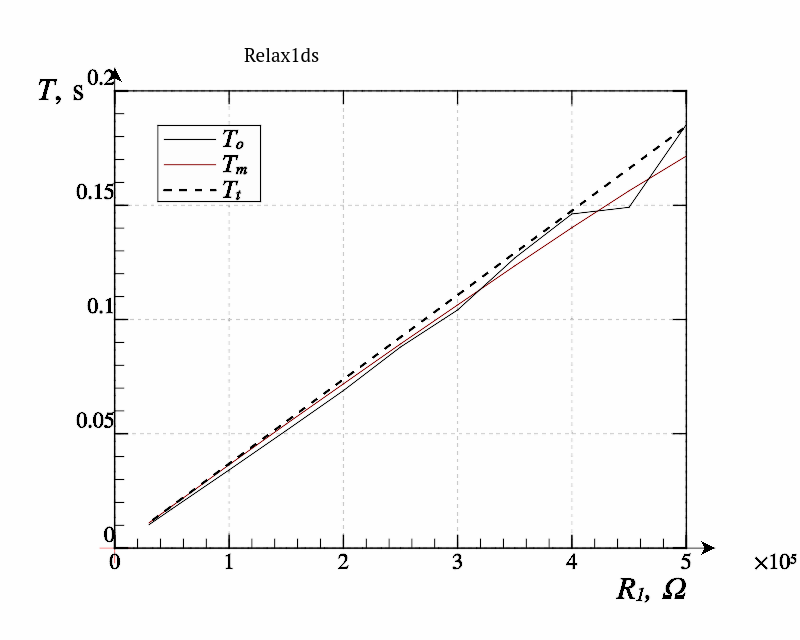
\includegraphics[width=0.6\textwidth]{p/relax1ds_read_cmp-p_R1_T.png} }
  \caption{Зависимости $T(R_1)$ в реальном эксперименте ``relax1ds'', полученной в результате моделирования, и теоретической (\ref{atu:eq:T_u_relax})}
  \label{atu:f:relax1ds_read_cmp-p_R1_T}
\end{figure}

За исключением одной точки, разница между экспериментальными и модельными значениями
меньше, чем для системы ``relax1d''. При этом наблюдается малое,
но всё же заметное расхождение между теоретически и модельными значениями.
В первую очередь, это связано с тем, что модель, помимо явлений,
описанных в теоретическом приближении, учитывает также токи утечки,
что становится более заметным при росте $R_1$.


Аналогичным способом сравнить результаты экспериментов и численного моделирования
для системы из трёх связанных генераторов не представляется возможным.
Даже для сложно-периодического режима визуальное сравнение формы колебаний
не имеет смысла, а сложные спектры не дают возможности
получить и сравнить зависимости частоты от какого-либо параметра.
Практически единственным выходом является использование критериев идентификации,
которые будут рассмотрены далее. Тем не менее, в качестве грубой предварительной
проверки адекватности может служить опять-же визуальное сравнение зависимости формы
аттракторов от параметра, а также характерные особенности спектров.

Рассмотрим и сравним формы аттракторов для объекта ``relax3d'' и его модели
в случае слабо-связанного режима, при $R_b=\SI{10}{\kilo\ohm}$ (рис.~\ref{atu:f:relax3d_mo_v1v2v3m_03})

\begin{figure}[htb!]
  \centerline{
    \hfill
    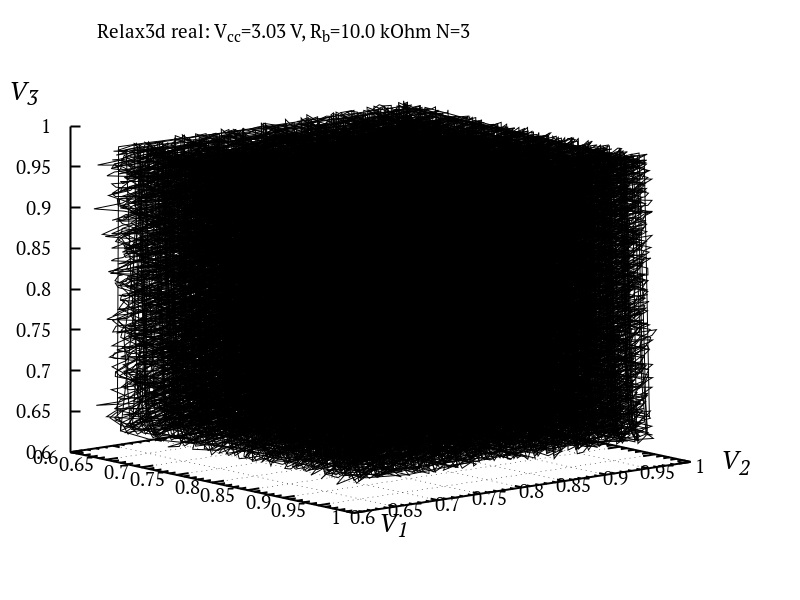
\includegraphics[width=0.48\textwidth]{p/relax3_v1v2v3_03.png}
    \hfill
    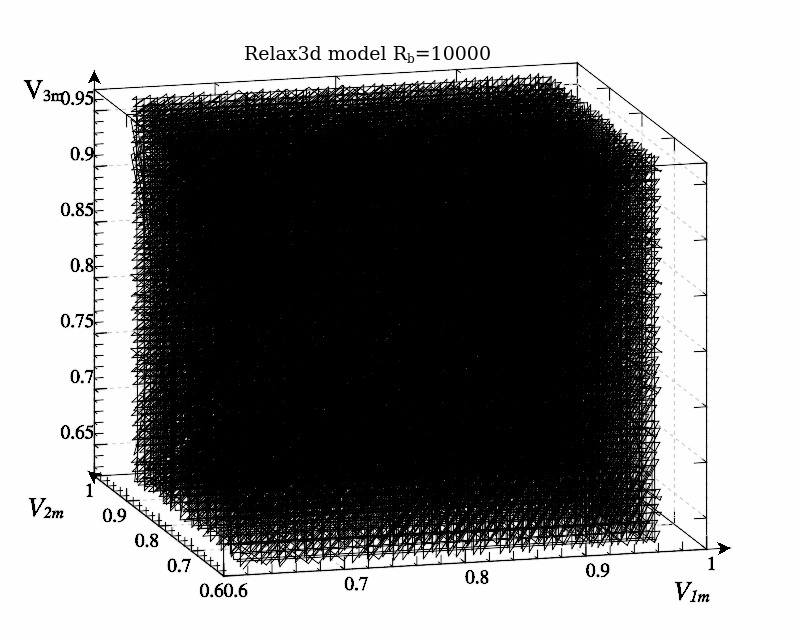
\includegraphics[width=0.48\textwidth]{p/relax3d_read_q-p_v1v2v3m_03a.png}
    \hfill
  }
  \caption{Аттракторы, полученные для объекта и модели при  $R_b=\SI{10}{\kilo\ohm}$}
  \label{atu:f:relax3d_mo_v1v2v3m_03}
\end{figure}

Формы аттракторов в обеих случаях имеют одинаковую плотно заполненную форму.
И у модели, и у объекта генераторы работают практически независимо,
сигналы имеют линейчатые спектры (рис.~\ref{atu:f:relax3d_mo_f_03}),
но более сложные, чем у независимых генераторов. Практически,
это проверка режима, близкого к независимым генераторам, и
результаты моделирования достаточно полно отображают этот факт.


\begin{figure}[htb!]
  \centerline{
    \hfill
    \includegraphics[width=0.48\textwidth]{p/relax3_f_03.png}
    \hfill
    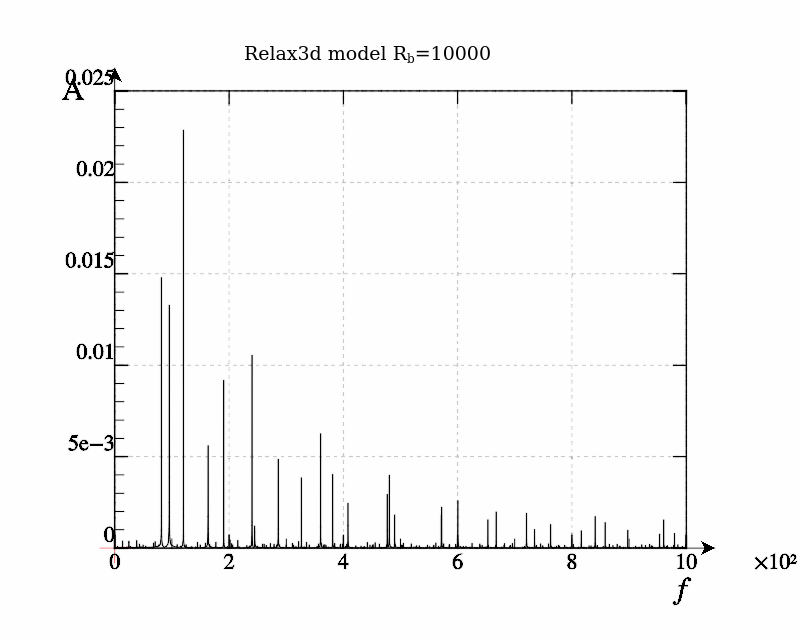
\includegraphics[width=0.48\textwidth]{p/relax3d_read_q-p_fm_03a.png}
    \hfill
  }
  \caption{Спектры сигнала $V_b(t)$ объекта и модели при  $R_b=\SI{10}{\kilo\ohm}$}
  \label{atu:f:relax3d_mo_f_03}
\end{figure}

Для хаотического режима для аттракторов наблюдается только
качественная схожесть (рис.~\ref{atu:f:relax3d_mo_v1v2v3m_17}).
При дальнейшем росте значения параметра
и у модели, и у объекта наблюдается вырожденное поведение.


\begin{figure}[htb!]
  \centerline{
    \hfill
    \includegraphics[width=0.48\textwidth]{p/relax3_v1v2v3_17.png}
    \hfill
    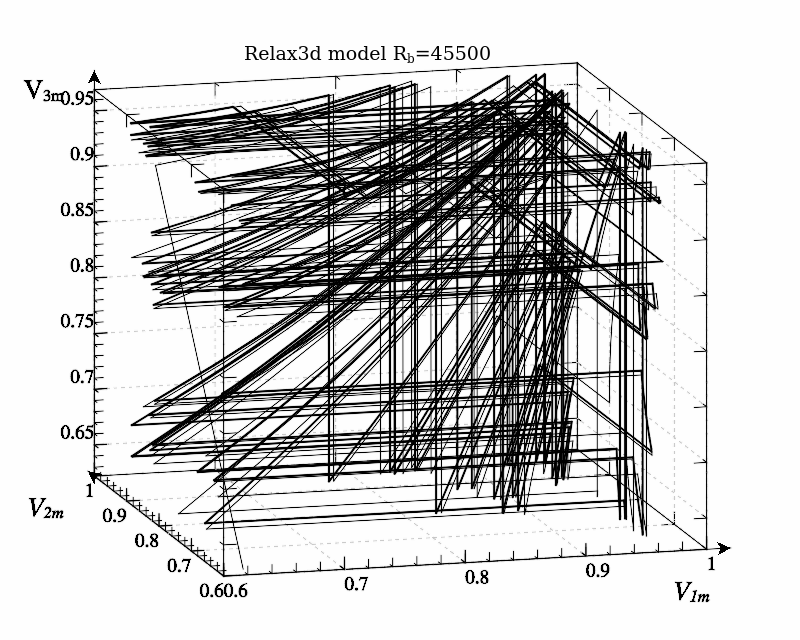
\includegraphics[width=0.48\textwidth]{p/relax3d_read_q-p_v1v2v3m_17a.png}
    \hfill
  }
  \caption{Аттракторы, полученные для объекта и модели при  $R_b=\SI{45.5}{\kilo\ohm}$}
  \label{atu:f:relax3d_mo_v1v2v3m_17}
\end{figure}

Спектры модели и объекта в этом режиме достаточно схожи именно из-за
своей сплошности и нерегулярности (рис.~\ref{atu:f:relax3d_mo_f_17}).
Выделить какую-то доминирующую частоту не представляется возможным,
хотя определённые пики на фоне сплошного спектра вполне различимы.

\begin{figure}[htb!]
  \centerline{
    \hfill
    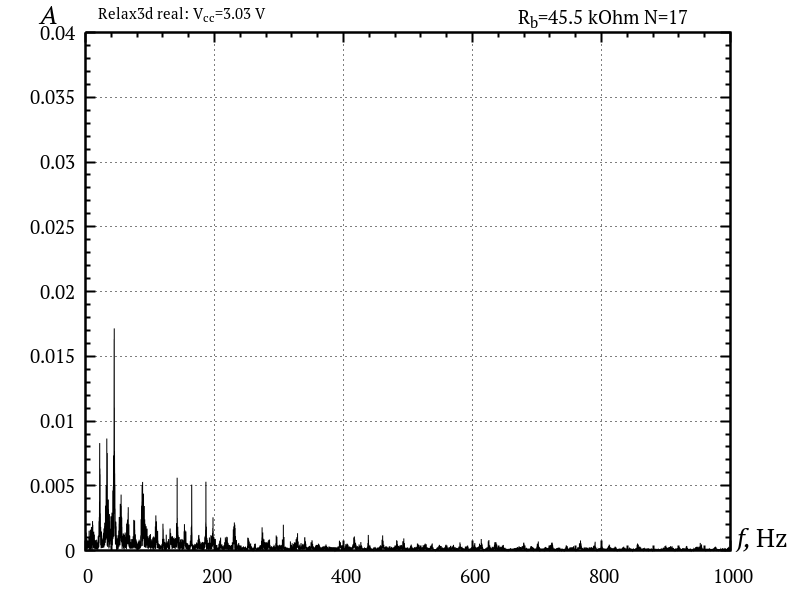
\includegraphics[width=0.48\textwidth]{p/relax3_f_17.png}
    \hfill
    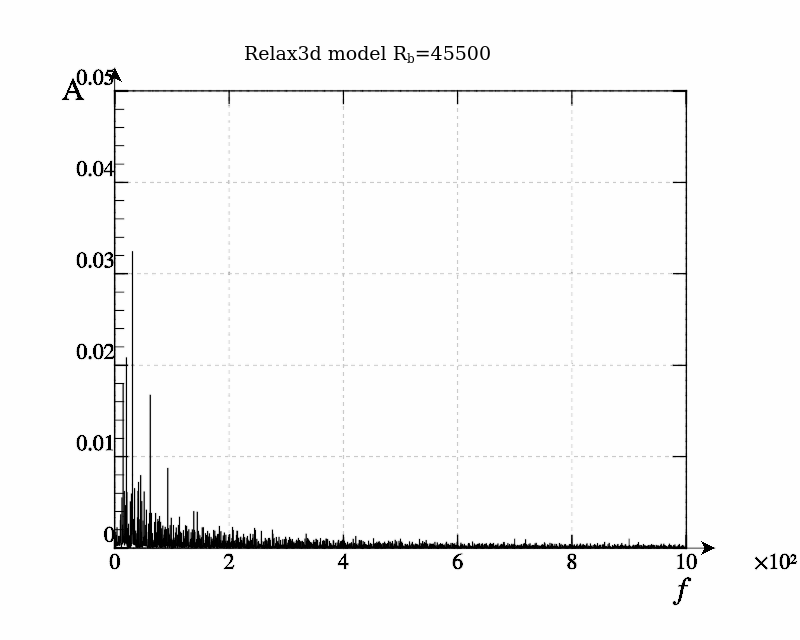
\includegraphics[width=0.48\textwidth]{p/relax3d_read_q-p_fm_17a.png}
    \hfill
  }
  \caption{Спектры сигнала $V_b(t)$ объекта и модели при  $R_b=\SI{45.5}{\kilo\ohm}$}
  \label{atu:f:relax3d_mo_f_17}
\end{figure}

Также следует отметить, что несмотря на похожесть аттракторов и спектров
объекта и модели при определённых значениях параметра,
моменты переключения между режимами, и само количество таких переключений
соблюдаются весьма приблизительно. Такое поведение характерно для систем хаотической динамики,
когда не только малые изменения в параметрах или начальных условиях приводят
к разбеганию траекторий, но и обычно пренебрежимо малые отличия в структуре модели приводят
к аналогичному результату.



\section{Критерии идентификации систем из трёх связанных релаксационных генераторов}

Рассмотрим возможные критерии для системы релаксационных
генераторов. В первую очередь имеет смысл
рассмотреть критерии, основанные на физических принципах.
Как уж было отмечено, использование в качестве критерия периода
колебаний неприменимо даже в случае сложно-периодического режима,
не говоря уже про хаотический.
Непосредственное применение энергетических критериев
для систем такого типа также не вполне обосновано ---
в системе такое соотношение между возможностями источника энергии
и потребителями (релаксационными элементами), что
потребление энергии лимитируется именно потребителями.
При этом моменты переключения определяются соответствующими разностями
потенциалов, следовательно, в первую очередь стоит рассматривать
интегральные величины, скорее всего --- каким-либо способом усреднённые значения
$V_b$, $V_1$, $V_2$, $V_3$.

Рассмотрим первый из кандидатов в критерии:
\begin{equation}
  q_{sv} = \overline{V_1+V_2+V_3} .
  \label{atu:eq:q_sv_relax}
\end{equation}


Как уже было отмечено (\ref{atu:eq:av_lin_relax},\ref{atu:eq:T_u_lin_relax})
эти величины непосредственно связаны с нелинейностью
зависимостей $V_i(t)$, и зависимость достаточно слабая.
При этом следует отметить достаточно неожиданный факт ---
при увеличении $R_b$, а следовательно ухудшении
возможностей источника питания, среднее напряжение
на релаксационных элементах растёт~(рис.~\ref{atu:f:relax3d_q}, \ref{atu:f:relax3ds_q}).
Это объясняется тем,
что при росте $R_b$ генераторы всё большую долю времени
затрачивают на ожидание непосредственно перед срабатыванием переключающего
элемента.

Таким образом, величину $q_{sv}$ можно использовать в качестве критерия,
но малый диапазон её изменения, вкупе с ошибками изменения,
препятствует созданию эффективной системы идентификации на этой основе.


Следующая величину, которую имеет смысл использовать в качестве критерия,
%
\begin{equation}
  q_{vb} = \overline{V_b} .
  \label{atu:eq:q_vb_relax}
\end{equation}
%
имеет непосредственную связь с идентифицируемым параметром $R_b$,
и, на первый взгляд, должна лучше подходить для
создания системы идентификации. Тем не менее,
анализ как реальных, так и модельных
зависимостей~(рис.~\ref{atu:f:relax3d_q}, \ref{atu:f:relax3ds_q}),
показывает, что данный критерий имеет преимущества при малых значениях $R_b$,
при которых связь между релаксационными элементами слаба,
и не хаотическое поведение не наблюдается. На первый взгляд,
это может быть связано о обратной зависимостью $q_{vb}(R_b)$,
и применение критерия вида
%
\begin{equation}
  q_{hv} = \frac{1}{\overline{V_b}} .
  \label{atu:eq:q_hb_relax}
\end{equation}
может исправить ситуацию. Тем не менее,
как результаты моделирования, так и натурный эксперимент
показывают, что это не так. Нелинейная
зависимость среднего тока через элемент
от среднего падения напряжения не даёт возможности
эффективно использовать $q_{hv}$.

Рассмотрим комбинированный критерий
\begin{equation}
  q_{rv} = \frac{\overline{V_1+V_2+V_3}}{\overline{V_b}}.
  \label{atu:eq:q_rv_relax}
\end{equation}


Анализ полученных зависимостей ~(рис.~\ref{atu:f:relax3d_q}, \ref{atu:f:relax3ds_q})
даёт основания полагать, что данный критерий --- лучший среди рассмотренных.
Более того, он является безразмерным, что является важным свойством критерия ---
скорее всего, при изменении параметров системы параметры системы
идентификации скорее всего не придётся перенастраивать.

\begin{figure}[htb!]
  \centerline{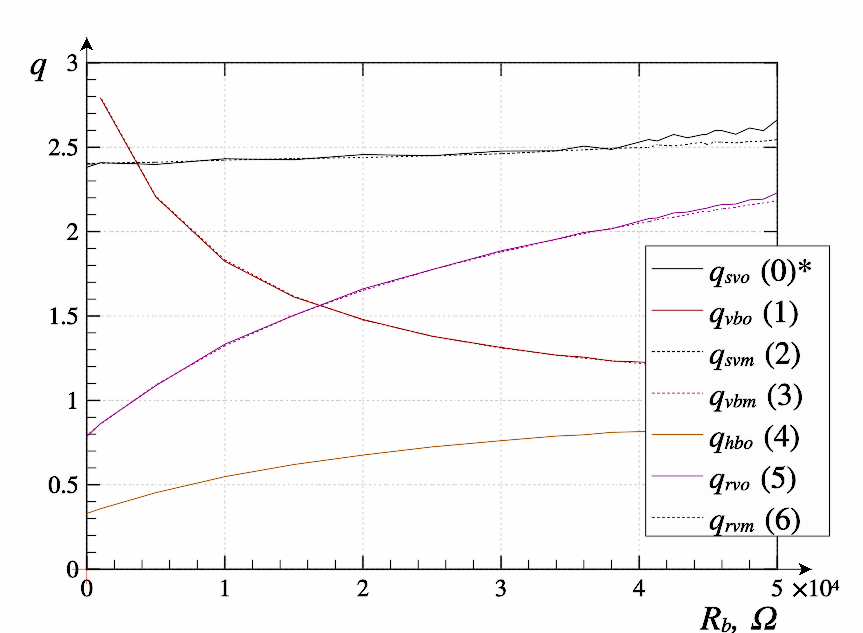
\includegraphics[width=0.7\textwidth]{p/relax3d_read_q-p_q1.png} }
  \caption{Зависимости для рассматриваемых критериев идентификации для системы релаксационных генераторов на паре комплиментарных транзисторов}
  \label{atu:f:relax3d_q}
\end{figure}

\begin{figure}[htb!]
  \centerline{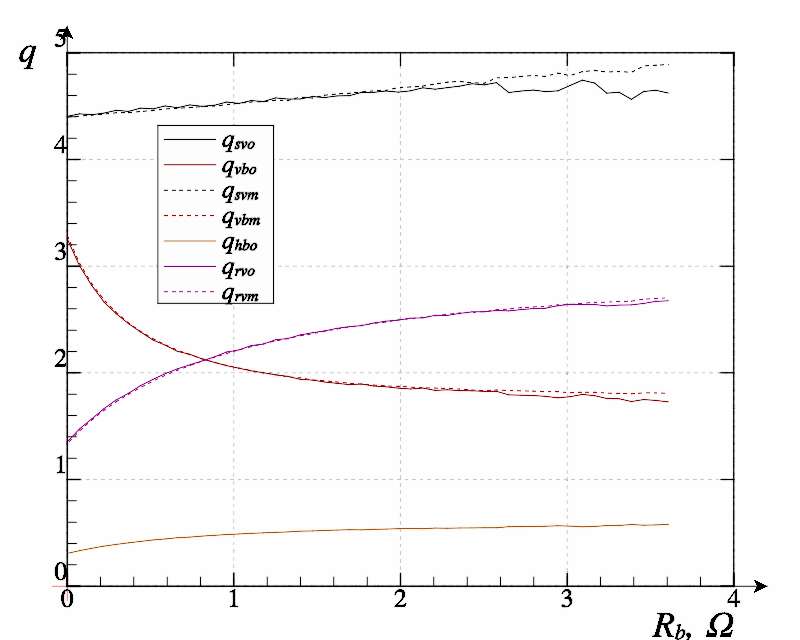
\includegraphics[width=0.7\textwidth]{p/relax3ds_read_q-p_q1.png} }
  \caption{Зависимости для рассматриваемых критериев идентификации для системы релаксационных генераторов на триггерах Шмидта}
  \label{atu:f:relax3ds_q}
\end{figure}

На представленных графиках приведены зависимости рассматриваемых критериев
как для реальных физических экспериментов (сплошные линии),
так и полученные в результате численного моделирования (штриховые линии).
Близость соответствующих кривых свидетельствует
о достаточной адекватности применяемых моделей.
Наибольшие отличия наблюдаются в правой части графиков, где существенными
явлениями являются токи утечки, имеющие нелинейную зависимость от разности потенциалов.
В этих местах прогнозируется рост систематической ошибки идентификации.
Тем не менее, несмотря на эти недостатки, общий вид этих зависимостей
даёт всё основания предполагать возможность построения работоспособной системы идентификации.


\section{Идентификация параметра системы из трёх связанных релаксационных генераторов}

Для проверки работоспособности и анализа
характеристик предлагаемых систем идентификации
были собраны соответствующие схемы.

Для обеспечения нестационарности параметра $R_b$
в качестве дополнительного сопротивления,
подключенного к шине питания через разъемы
P7~(рис.~\ref{atu:f:relax3d_schem}) и
P5~(рис.~\ref{atu:f:relax3ds_schem})
цифрового управляемого потенциометра CAT5171.
Данный электронный компонент представляет собой
управляемую по протоколу I2C сборку подключаемых резисторов.
Обеспечивается 256 значений управляемого сопротивления,
причём, согласно документации, гарантируется достаточная интегральная и
дифференциальная линейность зависимости сопротивления
от переданного кода: соответственно 2 и 1 младших разряда.
Температурная стабильность составляет 100~ppm/${}\SI{}{\celsius} $.
Из недостатков следует отметить значительный разброс полного сопротивления
относительно номинала (20~\%). В исследовательских
задачах этот недостаток нивелируется предварительной калибровкой.
Время установления после передачи требуемого значения составляет порядка
$\SI{20}{\micro\second}$,
что превышает время передачи. В свою очередь,
для рассматриваемой задачи задачи требуемое время
переключения --- от сотни миллисекунд до единиц секунд.

Для управления цифровым потенциометром в программе микроконтроллера была выделена
отдельная задача FreeRTOS. Для этой задачи задавалось
минимальное и максимальное значение кода сопротивления,
и требуемое время переключения в миллисекундах.
Затраты времени, требуемые для собственно переключения,
компенсировались на каждой итерации.
Основная задача, обеспечивающая получение отсчётов с АЦП,
синхронизировала начало своей работы
с моментом переключения цифрового потенциометра.
Анализ временных затрат, как и последующая работа системы,
показали, что времени микропроцессора достаточно (с учётом использования DMA)
для выполнения как указанных задач, так и служебных.
Во время записи результатов задача, отвечающая
за переключение сопротивления, останавливалась.

С учётом результатов предварительных исследований,
для каждой из рассматриваемой схемной реализации было выбраны
диапазоны изменения сопротивления таким образом, что бы
с одной стороны,
достаточно полно покрыть рабочий диапазон изменения параметра.
С другой --- для того, что бы при переключении были реализованы
различные режимы работы генератора.

В качестве методов идентификации для обеих систем был выбран набор
``FAlvn5.3z''. Таким образом исследовались различные способы оценивания экстремума
при одной и той же динамике агентов ансамбля.
На каждом из рисунков, иллюстрирующих процесс идентификации,
левый график показывает динамику агентов, а правый --- полученные
значения идентифицируемого параметра для различный способов:
$p_{ge}$, $p_{le}$, $p_{ee}$.
При моделировании процесса идентификации в программе ``qontrol''(рис.~\ref{atu:f:relax3d_id_qontrol})
в качестве данных с объекта использовались реальные данные,
записанные в файлы, которые служили источником данных.

\begin{figure}[htb!]
  \centerline{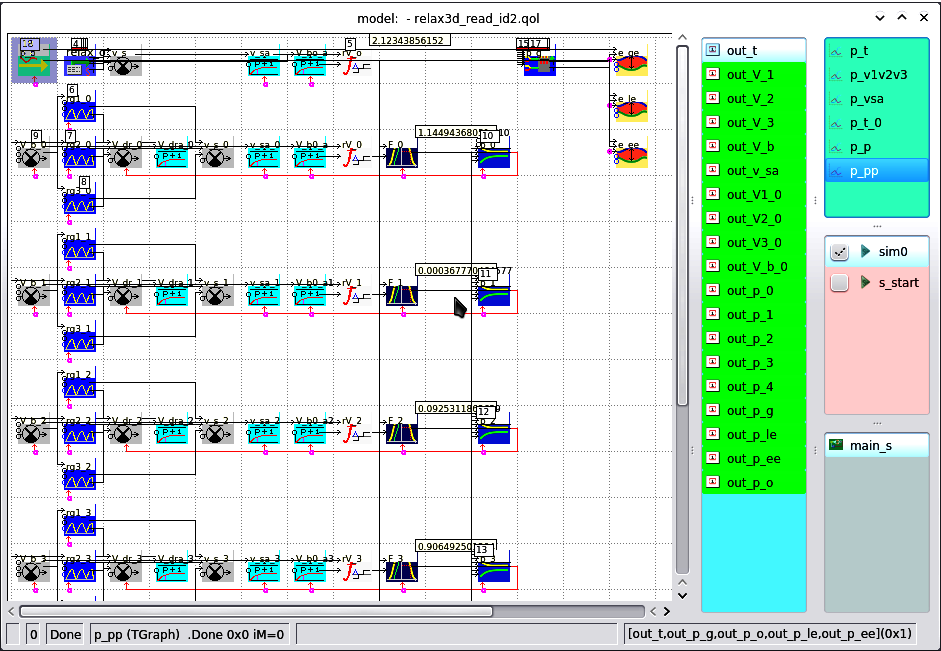
\includegraphics[width=0.9\textwidth]{p/relax3d_id_qontrol.png} }
  \caption{Модель системы идентификации для генератора ``relax3d'' в программе ``qontrol'' с использованием данных физического эксперимента}
  \label{atu:f:relax3d_id_qontrol}
\end{figure}

Для системы ``'relax3d' представлены результаты трех экспериментов,
каждый из которых заключался в получении данных
(отсчётов $V_b(t)$, $V_1(t)$, $V_2(t)$, $V_3(t)$) с реального генератора,
с последующим моделированием процесса идентификации в программе ``qontrol''.

Параметры первого эксперимента для системы ``relax3d'':
%
\begin{equation}
  \begin{array}{c}
    R_{b,\min} = \SI{30.0}{\kilo\ohm};
    \;
    R_{b,\max} = \SI{45.0}{\kilo\ohm};
    \;
    T_{R_b} = \SI{1.000}{\second};
  \\
    R_b(t) = \SI{37.5}{\kilo\ohm} + \SI{7.5}{\kilo\ohm} \cdot \sin( \pi ( t + 5.47 ) ).
  \end{array}
  \label{atu:eq:relax3d_test1_cond}
\end{equation}

\begin{figure}[htb!]
  \centerline{
    \includegraphics[width=0.48\textwidth]{p/relax3d_read_id2-p_p_00.png}
    \hfill
    \includegraphics[width=0.48\textwidth]{p/relax3d_read_id2-p_pp_00.png}
  }
  \caption{Процесс идентификации системы ``relax3d'' при условиях \ref{atu:eq:relax3d_test1_cond} (первый эксперимент)}
  \label{atu:f:relax3d_id_1}
\end{figure}

Результаты моделирования процесса идентификации в первом эксперименте~(рис.~\ref{atu:f:relax3d_id_1})
показывают, что система предложенная система идентификации оказалась работоспособной.
При этом следует отметить, что в первом эксперименте использовалась максимальная
амплитуда изменения параметра, следовательно основной вклад вносят ``крайние'' агенты,
наиболее подверженные влиянию границ рабочей области, тем не менее,
были получены вполне удовлетворительные результаты.
Визуально наилучшие результаты были получены при использовании $p_{ge}$ и $p_{le}$,
при использовании которых были получены практически совпадающие результаты.
Использование $p_{ee}$ приводит большей статической ошибке идентификации на верхнем пределе.
Тем не менее, средние относительные ошибки идентификации достаточно близки.
Более того, эта ошибку минимальна именно при использовании $p_{ee}$.



Параметры второго эксперимента для системы ``relax3d'':
%
\begin{equation}
  \begin{array}{c}
    R_{b,\min} = \SI{30.0}{\kilo\ohm};
    \;
    R_{b,\max} = \SI{42.0}{\kilo\ohm};
    \;
    T_{R_b} = \SI{1.000}{\second};
  \\
    R_b(t) = \SI{36.0}{\kilo\ohm} + \SI{6.0}{\kilo\ohm} \cdot \sin( \pi ( t + 1.33 ) ).
  \end{array}
  \label{atu:eq:relax3d_test2_cond}
\end{equation}

\begin{figure}[htb!]
  \centerline{
    \includegraphics[width=0.48\textwidth]{p/relax3d_read_id2-p_p_01.png}
    \hfill
    \includegraphics[width=0.48\textwidth]{p/relax3d_read_id2-p_pp_01.png}
  }
  \caption{Процесс идентификации системы ``relax3d'' при условиях \ref{atu:eq:relax3d_test2_cond} (второй эксперимент)}
  \label{atu:f:relax3d_id_2}
\end{figure}

Второй эксперимент отличается меньшей амплитудой изменения параметра.
При этом в целом были получены немного худшие результаты~(рис.~\ref{atu:f:relax3d_id_2}),
чем в предыдущем эксперименте,
проявившиеся в заметной статической ошибке идентификации как на верхнем,
так и на нижнем пределах. Это несколько удивительно, если учесть
тот факт, что нижние пределы в этих экспериментах совпадают.
Скорее всего, это было связано с неконтролируемыми помехами
в процессе измерения. Тем не менее, в целом результаты вполне удовлетворительны.



Параметры третьего эксперимента для системы ``relax3d'':
%
\begin{equation}
  \begin{array}{c}
    R_{b,\min} = \SI{30.0}{\kilo\ohm};
    \;
    R_{b,\max} = \SI{40.0}{\kilo\ohm};
    \;
    T_{R_b} = \SI{1.000}{\second};
  \\
    R_b(t) = \SI{35.0}{\kilo\ohm} + \SI{5.0}{\kilo\ohm} \cdot \sin( \pi ( t + 4.33 ) ).
  \end{array}
  \label{atu:eq:relax3d_test3_cond}
\end{equation}

\begin{figure}[htb!]
  \centerline{
    \includegraphics[width=0.48\textwidth]{p/relax3d_read_id2-p_p_02.png}
    \hfill
    \includegraphics[width=0.48\textwidth]{p/relax3d_read_id2-p_pp_02.png}
  }
  \caption{Процесс идентификации системы ``relax3d'' при условиях \ref{atu:eq:relax3d_test3_cond} (третий эксперимент)}
  \label{atu:f:relax3d_id_3}
\end{figure}

Третий эксперимент
характеризовался минимальной амплитудой изменения параметра,
и продемонстрировал визуально лучшие результаты~(рис.~\ref{atu:f:relax3d_id_3}).
Большие численные значения относительной ошибки
вызваны именно меньшей амплитудой изменения параметра,
т.е. абсолютная ошибка нормировалась на меньшую величину.




Для системы ``'relax3ds' представлены результаты четырёх экспериментов,
проведённых в аналогичных условиях.

Параметры первого эксперимента для системы ``relax3ds'':
%
\begin{equation}
  \begin{array}{c}
    R_{b,\min} = \SI{5.15}{\kilo\ohm};
    \;
    R_{b,\max} = \SI{24.84}{\kilo\ohm};
    \;
    T_{R_b} = \SI{1.000}{\second};
  \\
    R_b(t) = \SI{15.00}{\kilo\ohm} + \SI{9.84}{\kilo\ohm} \cdot \sin( \pi ( t + 1 ) ).
  \end{array}
  \label{atu:eq:relax3ds_test1_cond}
\end{equation}


\begin{figure}[htb!]
  \centerline{
    \includegraphics[width=0.48\textwidth]{p/relax3ds_read_id2_0-p_p.png}
    \hfill
    \includegraphics[width=0.48\textwidth]{p/relax3ds_read_id2_0-p_pp.png}
  }
  \caption{Процесс идентификации системы ``relax3ds'' при условиях \ref{atu:eq:relax3ds_test1_cond} (первый эксперимент)}
  \label{atu:f:relax3ds_id_0}
\end{figure}

Условия этого эксперимента были выбраны так, что бы проверить работоспособность
на близкой к максимальной амплитуде изменения параметра.
Результаты моделирования показывают~(рис.~\ref{atu:f:relax3ds_id_0}), что все три подхода к определению
$p_e$ позволяют в этих условиях получить работоспособную систему идентификации.
Время реакции на переключение составляет 0.3--0.4~s. При этом обнаруживается
различие методов на верхнем и нижнем пределах:
$p_{ge}$ и $p_{le}$ обеспечивают максимальную точность идентификации на нижнем пределе,
а $p_{ee}$ --- на верхнем. Суммарно ошибки идентификации для всех трех методов
практически идентичны.


Параметры второго эксперимента для системы ``relax3ds'':
%
\begin{equation}
  \begin{array}{c}
    R_{b,\min} = \SI{9.94}{\kilo\ohm};
    \;
    R_{b,\max} = \SI{23.00}{\kilo\ohm};
    \;
    T_{R_b} = \SI{1.000}{\second};
  \\
    R_b(t) = \SI{16.47}{\kilo\ohm} + \SI{6.53}{\kilo\ohm} \cdot \sin( \pi ( t + 1 ) ).
  \end{array}
  \label{atu:eq:relax3ds_test2_cond}
\end{equation}

\begin{figure}[htb!]
  \centerline{
    \includegraphics[width=0.48\textwidth]{p/relax3ds_read_id2_1-p_p.png}
    \hfill
    \includegraphics[width=0.48\textwidth]{p/relax3ds_read_id2_1-p_pp.png}
  }
  \caption{Процесс идентификации системы ``relax3ds'' при условиях \ref{atu:eq:relax3ds_test2_cond} (второй эксперимент)}
  \label{atu:f:relax3ds_id_1}
\end{figure}

Второй эксперимент, с меньшей амплитудой изменения параметра,
при сохранении работоспособности, и, в целом,
немного меньшими ошибками идентификации,
проявляет несколько иную картину~(рис.~\ref{atu:f:relax3ds_id_1}):
верхний предел уверенно определяется всеми методами,
а нижний лучше идентифицируется при использовании
$p_{ee}$.


Параметры третьего эксперимента для системы ``relax3ds'':
%
\begin{equation}
  \begin{array}{c}
    R_{b,\min} = \SI{13.06}{\kilo\ohm};
    \;
    R_{b,\max} = \SI{27.97}{\kilo\ohm};
    \;
    T_{R_b} = \SI{1.000}{\second};
  \\
    R_b(t) = \SI{20.51}{\kilo\ohm} + \SI{7.45}{\kilo\ohm} \cdot \sin( \pi ( t + 1 ) ).
  \end{array}
  \label{atu:eq:relax3ds_test3_cond}
\end{equation}

\begin{figure}[htb!]
  \centerline{
    \includegraphics[width=0.48\textwidth]{p/relax3ds_read_id2_2-p_p.png}
    \hfill
    \includegraphics[width=0.48\textwidth]{p/relax3ds_read_id2_2-p_pp.png}
  }
  \caption{Процесс идентификации системы ``relax3ds'' при условиях \ref{atu:eq:relax3ds_test3_cond} (третий эксперимент)}
  \label{atu:f:relax3ds_id_2}
\end{figure}

В данном эксперименте среднее значение идентифицируемого параметра
сдвинуто в сторону больших значений. И, как следствие,
при идентификации на верхнем пределе ошибка максимальна~(рис.~\ref{atu:f:relax3ds_id_2}).
В первую очередь, это связана с тем, что на этом участке
чувствительность критерия к изменению параметра минимальна.
Играет свою роль и увеличение ошибок при моделировании
режима с минимальным энергопотреблением.
Тем не менее, даже в этих условиях методы сохраняют работоспособность.


Параметры четвёртого эксперимента для системы ``relax3ds'':
%
\begin{equation}
  \begin{array}{c}
    R_{b,\min} = \SI{5.52}{\kilo\ohm};
    \;
    R_{b,\max} = \SI{18.40}{\kilo\ohm};
    \;
    T_{R_b} = \SI{1.000}{\second};
  \\
    R_b(t) = \SI{11.96}{\kilo\ohm} + \SI{6.44}{\kilo\ohm} \cdot \sin( \pi ( t + 1 ) ).
  \end{array}
  \label{atu:eq:relax3ds_test4_cond}
\end{equation}

\begin{figure}[htb!]
  \centerline{
    \includegraphics[width=0.48\textwidth]{p/relax3ds_read_id2_3-p_p.png}
    \hfill
    \includegraphics[width=0.48\textwidth]{p/relax3ds_read_id2_3-p_pp.png}
  }
  \caption{Процесс идентификации системы ``relax3ds'' при условиях \ref{atu:eq:relax3ds_test4_cond}}
  \label{atu:f:relax3ds_id_3}
\end{figure}

Результаты четвёртого эксперименты ещё раз
подтверждают работоспособность предложенных методов.
В целом, в различных экспериментах различные методы
показывали лучшие результаты, однако в целом результаты
примерно равнозначные. Практически невозможно в данных условиях выбрать лучший
метод, с учётом того факта, что значения идентифицируемого
параметра заранее не известны.




\section{Выводы по разделу \thechapter}

В целом, результаты экспериментов,
моделирования динамики систем связанных релаксационных генераторов
и процессов идентификации параметра $R_b$, определяющего величину этой связи,
позволяют сделать следующие выводы:

\begin{itemize}

  \item
    Система из трех связанных по цепи питания релаксационных генераторов,
    в зависимости от величины этой связи, может
    проявлять как практически независимые колебания,
    так и сложно-периодическую и хаотическую динамику.


  \item
    Вид аттракторов этой системы в случае слабо-связанных колебаний,
    является достаточно необычным: практически полностью заполненный
    прямоугольный параллелепипед,
    а вид аттрактора в хаотических режимах не является
    модификацией аттракторов наиболее известных хаотических систем.


  \item
    Комбинированный критерий идентификации (\ref{atu:eq:q_rv_relax})
    обеспечивает наилучшее качество идентификации из рассмотренных.

  \item
    Системы мультиагентной идентификации ``FAlvn5.3z''
    продемонстрировали на реальных тестовых данных
    хорошую работоспособность.

  \item
    Зависимости удельных ошибок идентификации \Cmt{TODO}

  \item

\end{itemize}




